\documentclass[a4j]{jsarticle}
%
% 古いパッケージを自動チェック
% \RequirePackage[l2tabu, orthodox]{nag}
% \usepackage[all, warning]{onlyamsmath}
% 古いパッケージを自動チェック

%\usepackage{subcaption} %図の中に複数の図を入れる
\usepackage[top=30mm,bottom=30mm,left=25mm,right=25mm]{geometry}% 幅160mmの余り
\usepackage{url} %URLを表示する
\usepackage[dvipdfmx]{graphicx}
\usepackage[dvipdfmx]{color}
\usepackage[dvipdfmx]{hyperref}
\usepackage{pxjahyper}
\usepackage{verbatim}
\usepackage{amsmath}
\usepackage{subfig}
% \usepackage{subcaption}
\usepackage{textcomp}
\usepackage{url}
\usepackage{color}
\setcounter{tocdepth}{\maxdimen} %subsubsectionまで目次を表示する
\bibliographystyle{junsrt} %参照のスタイル

\title{\vspace{60mm} \large 卒業論文\vspace{10mm}\\ \LARGE\LaTeX での論文の書き方(論文のタイトル)\vspace{5mm}}
\author{\large 岐阜大学 教育学部 \\ \vspace{5mm}
\large 理科教育講座 物理学 \\ \vspace{5mm}
\large おなまえ}
\date{最終更新 \today}

% ドキュメント
\begin{document}
% タイトル
\maketitle
\thispagestyle{empty} %ページ番号を消す
\newpage %新しいページ
\tableofcontents %目次の表示
\newpage %新しいページ
\section*{アブストラクト}

\LaTeX とは、テキストベースで論文等を執筆するための組み版システムである。Microsoft Wordに対する利点は、図や表を入れる際に配置などを気にしなくても良いこと、参考文献などの管理がしやすいこと、数式が美しく表現できることなどが挙げられる。対して欠点としては、Microsoft Wordよりも取っつきにくいこと、ある程度はコマンドを覚える必要があること、そして卒業した後にあまり使う機会がないということが挙げられる。私は執筆にとにかく集中できるという理由で \LaTeX を使っているが、個人の好みを押しつけるつもりはない。

この文章は、修士論文と卒業論文を\LaTeX で書く人のために、\LaTeX の使い方を何度もググる必要がないようにまとめた文章である。論文としての書き方は厳密に正しくはないので注意してほしい。

講習前の準備として、README.md に書かれた準備は完了しただろうか。ここからは、準備が完了したことを前提に話を進めていくことにする。

論文の編集は Visual Studio Code (エディタ) + LaTeX Workshop (Visual Code内の拡張機能) を使うと便利である。Visual Studio Codeの設定ファイル (User Settings) に以下のコードを書いておけば、ファイルを編集し保存する度に自動的にコンパイルされる。ちなみに、ptex2pdfを2度実行しているのは目次や図表や参考文献などのリンク(番号)を2度目で生成しているからである。
\begin{verbatim}
"latex-workshop.latex.tools": [
    {
        "name": "ptex2pdf",
        "command": "ptex2pdf",
        "args": [
            "-l",
            "-ot",
            "-kanji=utf8",
            "-synctex=1",
            "-interaction=nonstopmode",
            "-shell-escape",
            "%DOCFILE%"
        ]
    }
],
"latex-workshop.latex.recipes": [
    {
        "name": "ptex2pdf",
        "tools": [
            "ptex2pdf",
            "ptex2pdf"
        ]
    }
],
\end{verbatim}

必須ではないが、Windowsユーザーの方は、PDF表示用にSumatraPDFをインストールすることをお勧めする。Visual Studio Code と SumatraPDFの組み合わせでは、SumatraPDFのオプションの逆順検索コマンドラインの設定で、\verb|"C:\Program Files\Microsoft VS Code\code.exe" -g "%f:%l"|などと書いておくと、PDFファイルの文章をクリックするとテキストファイルの元の文章の場所に飛ぶことができる。なお、\verb|code.exe|のパスは上記の限りではないので注意されたし。

bibtexを使う場合は \verb|pbibtex -kanji=utf8 filename| のようにコマンドを叩く。\verb|.tex| は必要ない。

\section*{講習会について}

講習会が開始する前に、README.md を読んで\LaTeX のインストールが完了していることを前提にしている。インストールには時間がかかるため、講習中にインストールを完了させるのは難しいだろう。講習会でよく質問して、よく理解して、LaTeXが難しそうならWordで書くのも個人的には有りだと思う。とにかく、自分に適した快適な執筆環境が構築できれば幸いである。

\section*{このファイルについて}
このファイルには、私がお勧めする設定は網羅している。不要なところを削除するなどして、論文を書き始めて欲しい。

\section*{著者について}

吉本 雅浩 (岐阜大学 教育学部)

\section*{ライセンス}

GNU General Public License (GNU GPL)

\newpage %新しいページ
\section{特殊文字について}
\subsection{メタ文字}
\LaTeX のメタ文字は以下の13種。これらは文中で直接使うことができない。
\begin{verbatim}
#, $, %, &, ~, _, ^, \, {, }, >, <, |, ¥
\end{verbatim}
以上の文字群は面倒だが次のように書く。最後の\verb|\\|は改行コードである。
\begin{verbatim}
\#, \$, \%, \&, \textasciitilde, \_, \textasciicircum, \textbackslash , \\
\{, \}, \verb|>|, \verb|<|, $|$, \textyen
\end{verbatim}
実際に書くと次のようになる。\\
\#, \$, \%, \&, \textasciitilde, \_, \textasciicircum, \textbackslash , \\
\{, \}, \verb|>|, \verb|<|, $|$, \textyen

\subsection{空白}
空白は主に4種類ある。次の3つである。ちなみに、数字と\%や角度を表す$^\circ$の間に空白は必要ない。\\
\verb|~|は改行されない空白で主に数字と単位の間や、図と\verb|\ref{}|の間に書く。\\
\verb|\| は半角1文字分の空白、\\
\verb|\quad|は全角分(半角2文字分)の空白、\\
\verb|\,|は小さい空白(正確には半角の1/3)である。
\subsection{改行・改ページ}
改行にはインデントあり、なし、縦方向のスペースの3種がある。\\
ただの空行 又は \verb|\par| でインデント"あり"の改行\\
\verb|\\| 又は \verb|\newline| でインデント"なし"の改行\\
\verb|\\*| 又は \verb|\newline*| で改行位置での改ページを禁止した改行\\
\verb|\vspace{10mm}|	縦方向のスペース、無理矢理なので多用しない。\\
\verb|\noindent| は文頭でインデントしたくない時に使う\\
\verb|\newpage| で改ページ、\verb|\clearpage| で全てのグラフ等を出力した後に改ページ
\subsection{ハイフンとダッシュ}
使い方を間違えやすいのがハイフンとダッシュ。
ハイフンとenダッシュと、emダッシュの3つがある。

\subsubsection{ハイフン}
ハイフンを一つで表現する。単語の途中で改行する場合(ただし \LaTeX  では自動でしてくれるので我々は何もしなくて良い)、または単語をつなげて形容詞を作る時に用いる。

\subsubsection{en ダッシュ}
ハイフンを二つで表現する。範囲を表す時に用いる。
英語においては範囲を表すのに~を使わない方がよいが、日本語の論文の場合は意味は通じるので構わないだろう。

\subsubsection{em ダッシュ}
ハイフン三つで表現する。文章中に句を挿入する時に用いる。前後にスペースを入れない。

\subsubsection{使用例}
\begin{itemize}
 \item I am twenty-two years old. (単語をつなげるハイフン) \verb|-|
 \item 〒770--8506 (電話や郵便番号のハイフン)  \verb|--|
 \item B4 -- M2の3年間所属しました。(範囲を表すen ダッシュ) \verb|--|
 \item The optics---i.e., objective lens, illuminator, and beam splitter---were designed. (挿入句を表すem ダッシュ) \verb|---|
 \item $(2016-2014+1)$年間所属しました。(引き算) \verb|$-$|
\end{itemize}
\clearpage
\section{図\label{sec:figure}}
\subsection{図の基本}
図はtexファイルの外に保存しておき、texファイルにその場所を指し示すコマンドを書けば挿入できる。ファイルはtexファイルがある場所からの相対パスで書くことが出来る。このサンプルでは全てのファイルを\verb|figs|というフォルダ内に保存してある。拡張子の前の.と間違えるので、パスの中に.を含めることはできない。

図が出現する場所はユーザー側がここに挿入したいという場所に必ずしも挿入されるわけではない。一般的に論文にでは図が文中に出てくるより前に来るか後に来るかは問われないため、特段気にする必要はない。\verb|[htbp]|はh=その場所に、t=ページの上部に、b=ページの下部に、p=独立したページにそれぞれ表示するように試す(私も正確な仕様は把握していない)。

本文中の図番号は、図中で指定したlabel名と対応し、図が出現する順番に自動で割り振られる。本文中には\verb|図\ref{fig:image}|と書き、図のキャプション内に\verb|\label{fig:image}|と書いておくと、\verb|fig:image|が目印となって番号が勝手に挿入される。

例えば、次のように\verb|result2.pdf|を挿入したとしよう。

\begin{verbatim}
\begin{figure}[htbp]
\centering
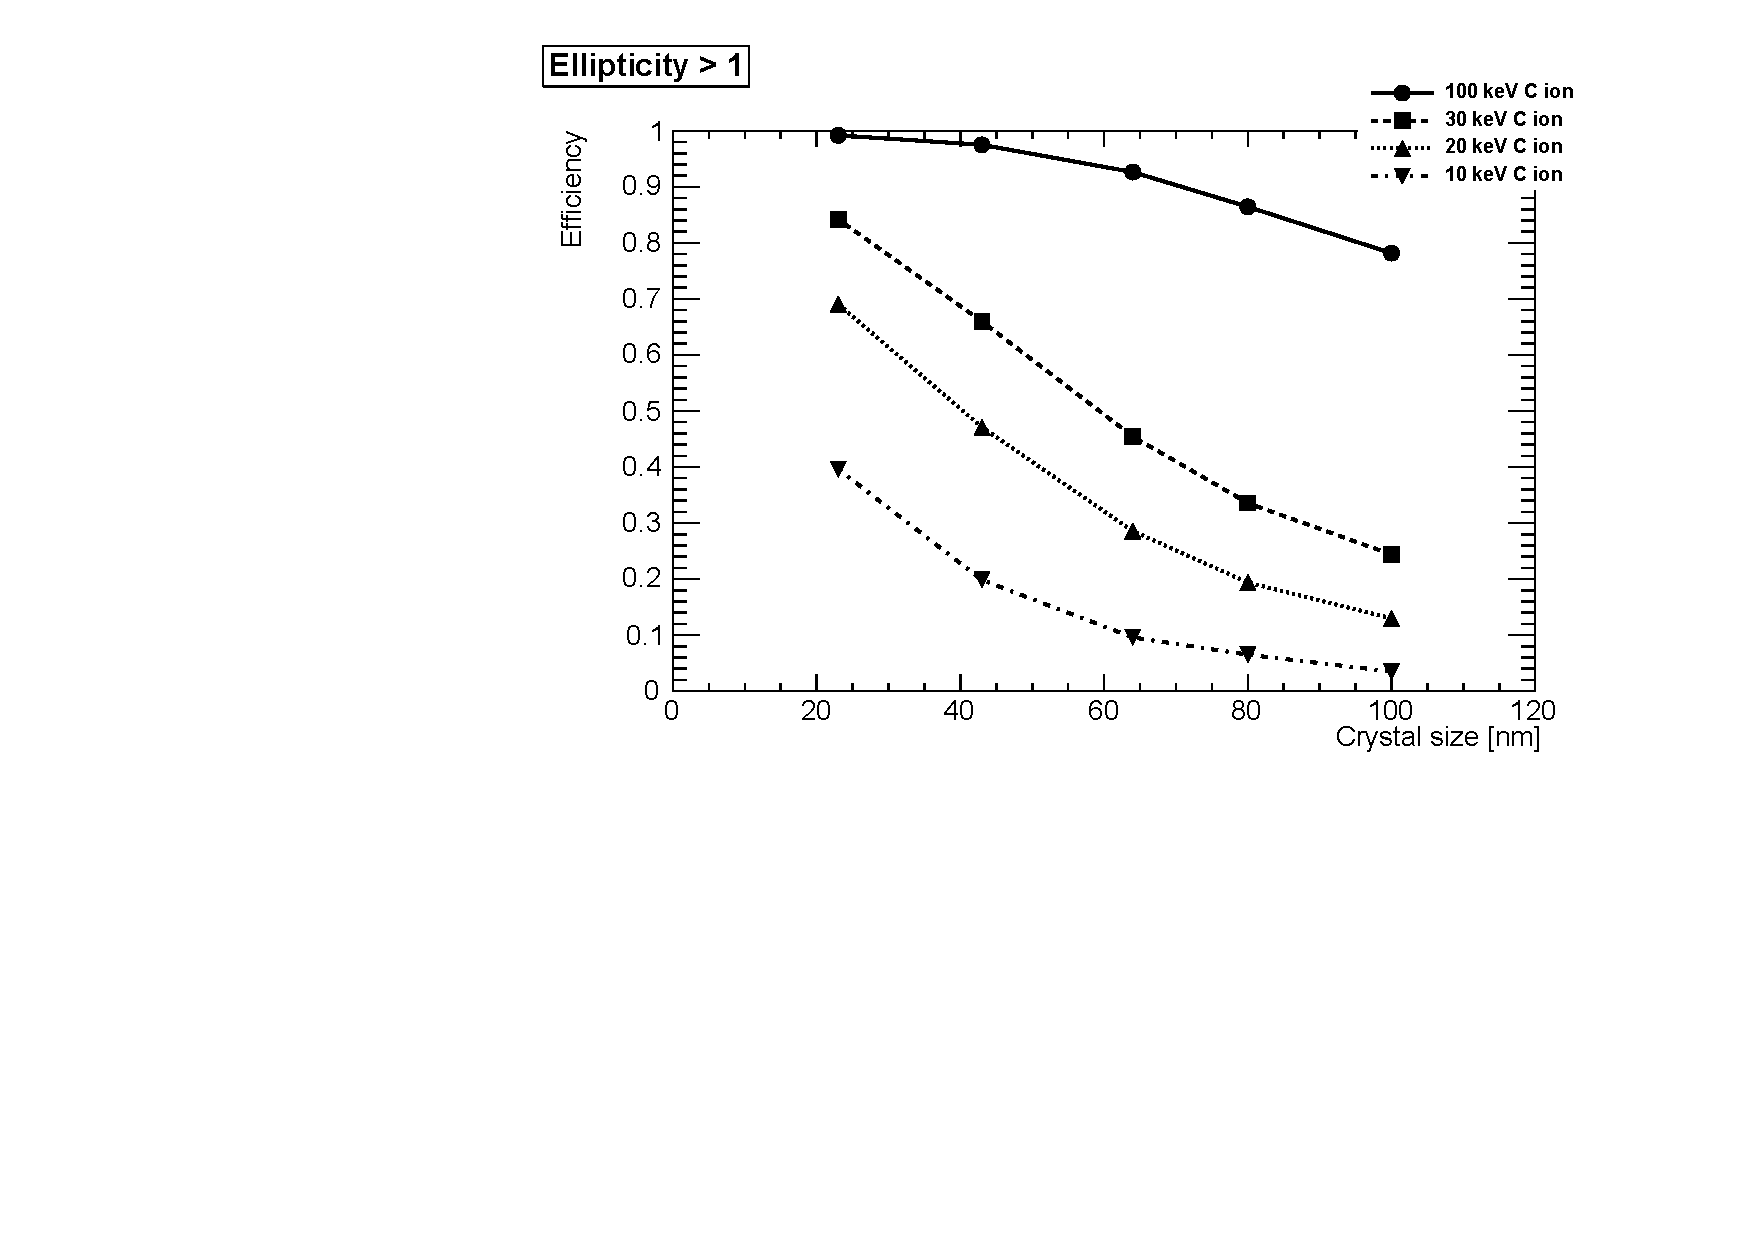
\includegraphics[width=70mm]{./figs/result2.pdf}
\caption{幅70mmで画像を表示する方法\label{fig:test_image}}
\end{figure}
\end{verbatim}

これを実際に描くと図~\ref{fig:test_image}のようになる。

\begin{figure}[htbp]
\centering
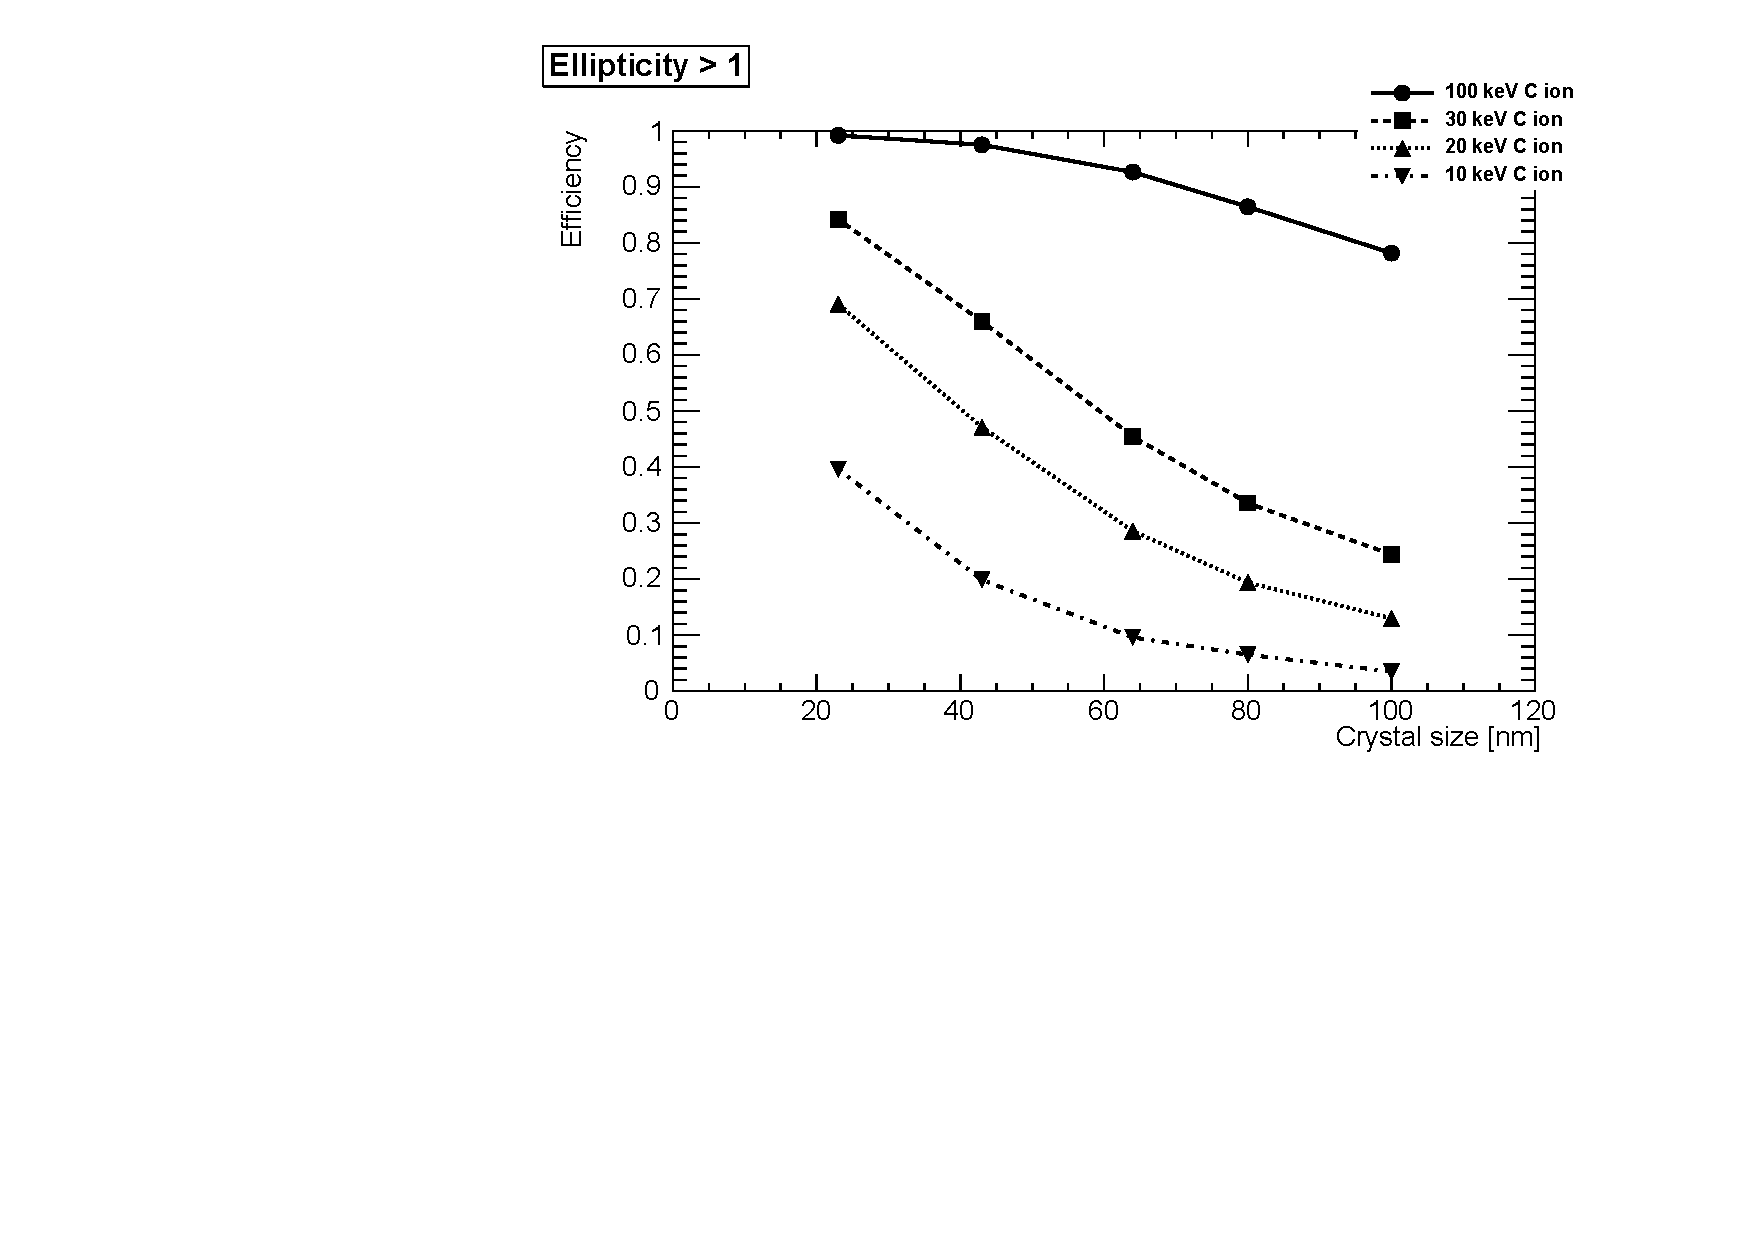
\includegraphics[width=70mm]{./figs/result2.pdf}
\caption{幅70mmで画像を表示する方法\label{fig:test_image}}
\end{figure}

画像のサイズの指定方法は、いくつかの方法がある。

\begin{verbatim}
width=100mm 幅をミリメートルで指定する方法
width=1.0\textwidth テキスト幅からの倍率で指定する方法
scale=0.2 画像やPDFファイルのサイズからの倍率を指定する方法
\end{verbatim}

\subsection{複数の図を表示}
複数の画像を一つの図に表示させる方法がある。図~\ref{fig:multi_images}で例を描画した。ソース次のとおり。
\begin{verbatim}
\begin{figure}[htbp]
\centering
\subfloat[0~degree]{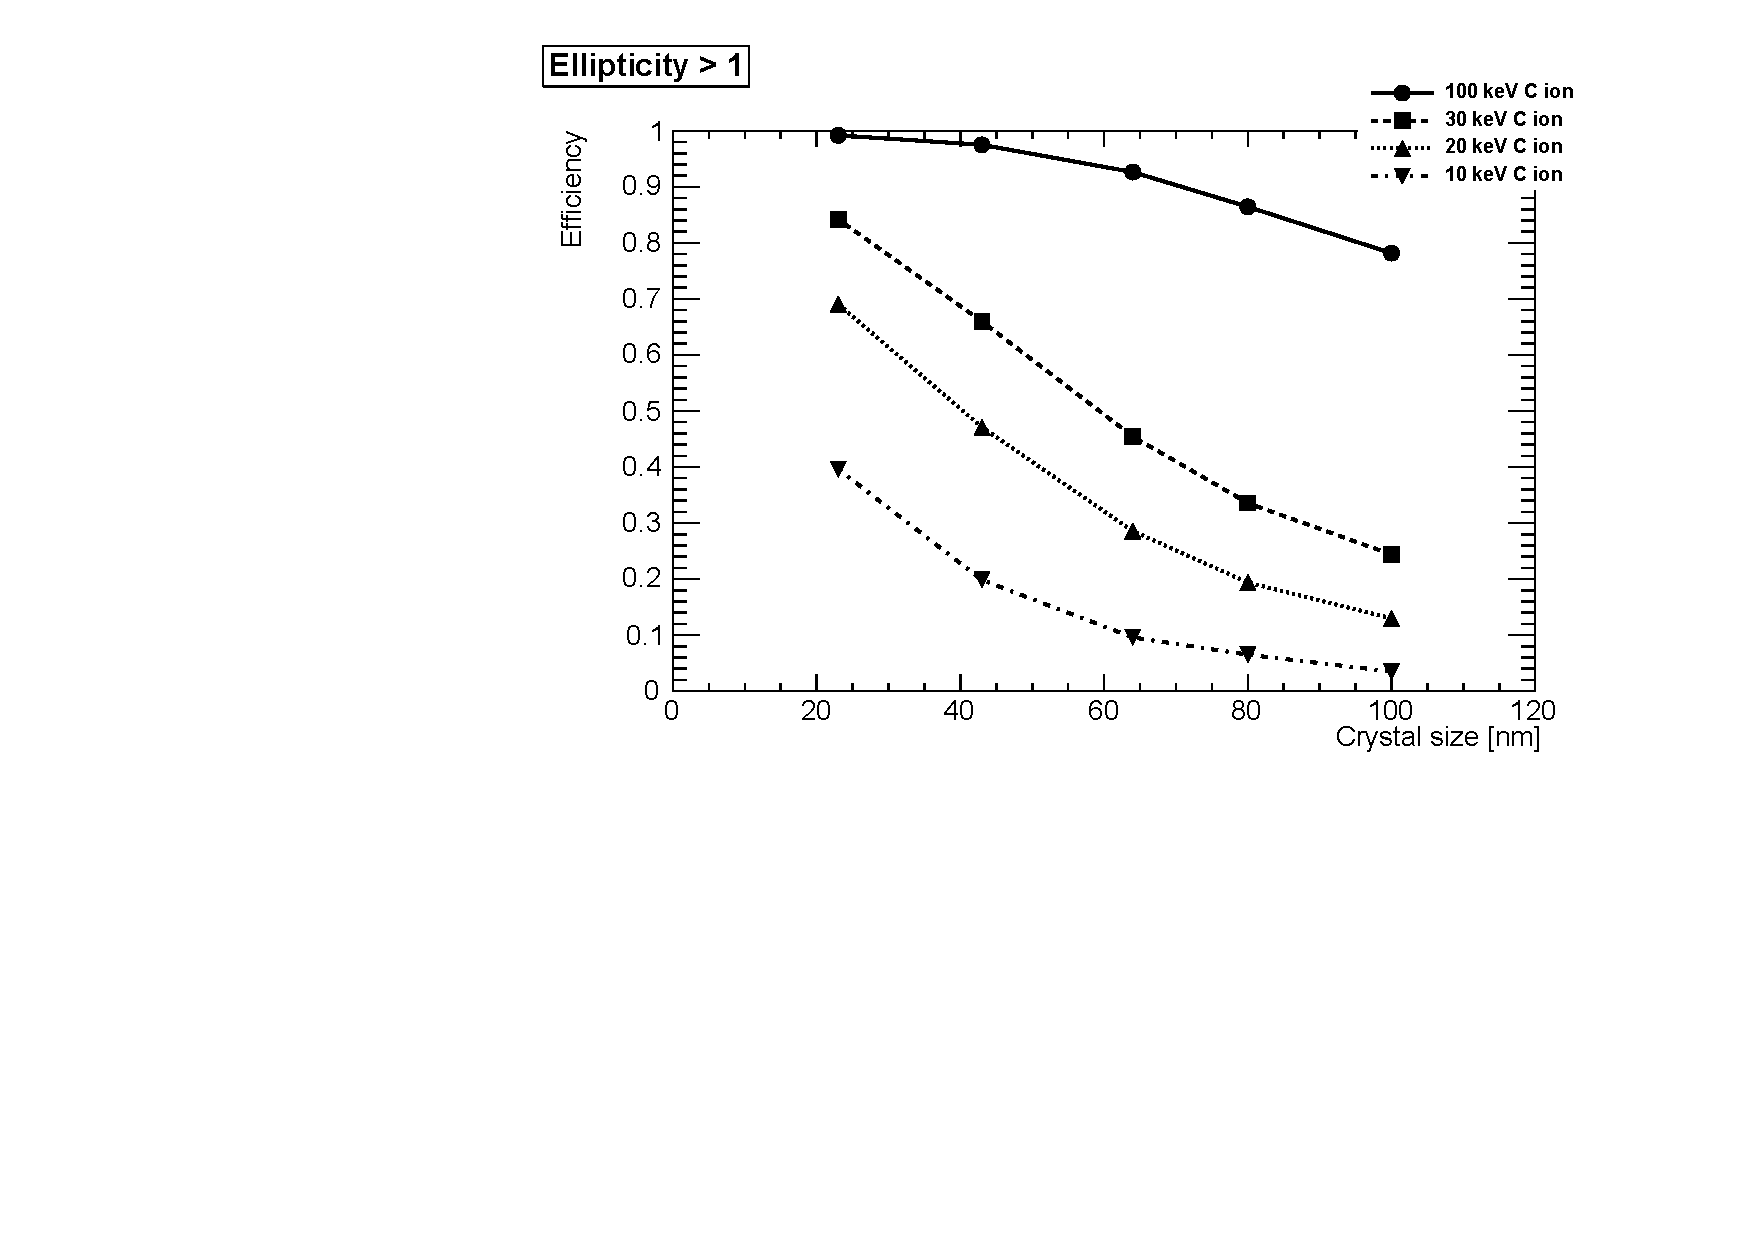
\includegraphics[angle=0,scale=0.2]{./figs/result2.pdf}}
\hspace{1em}
\subfloat[45~degree]{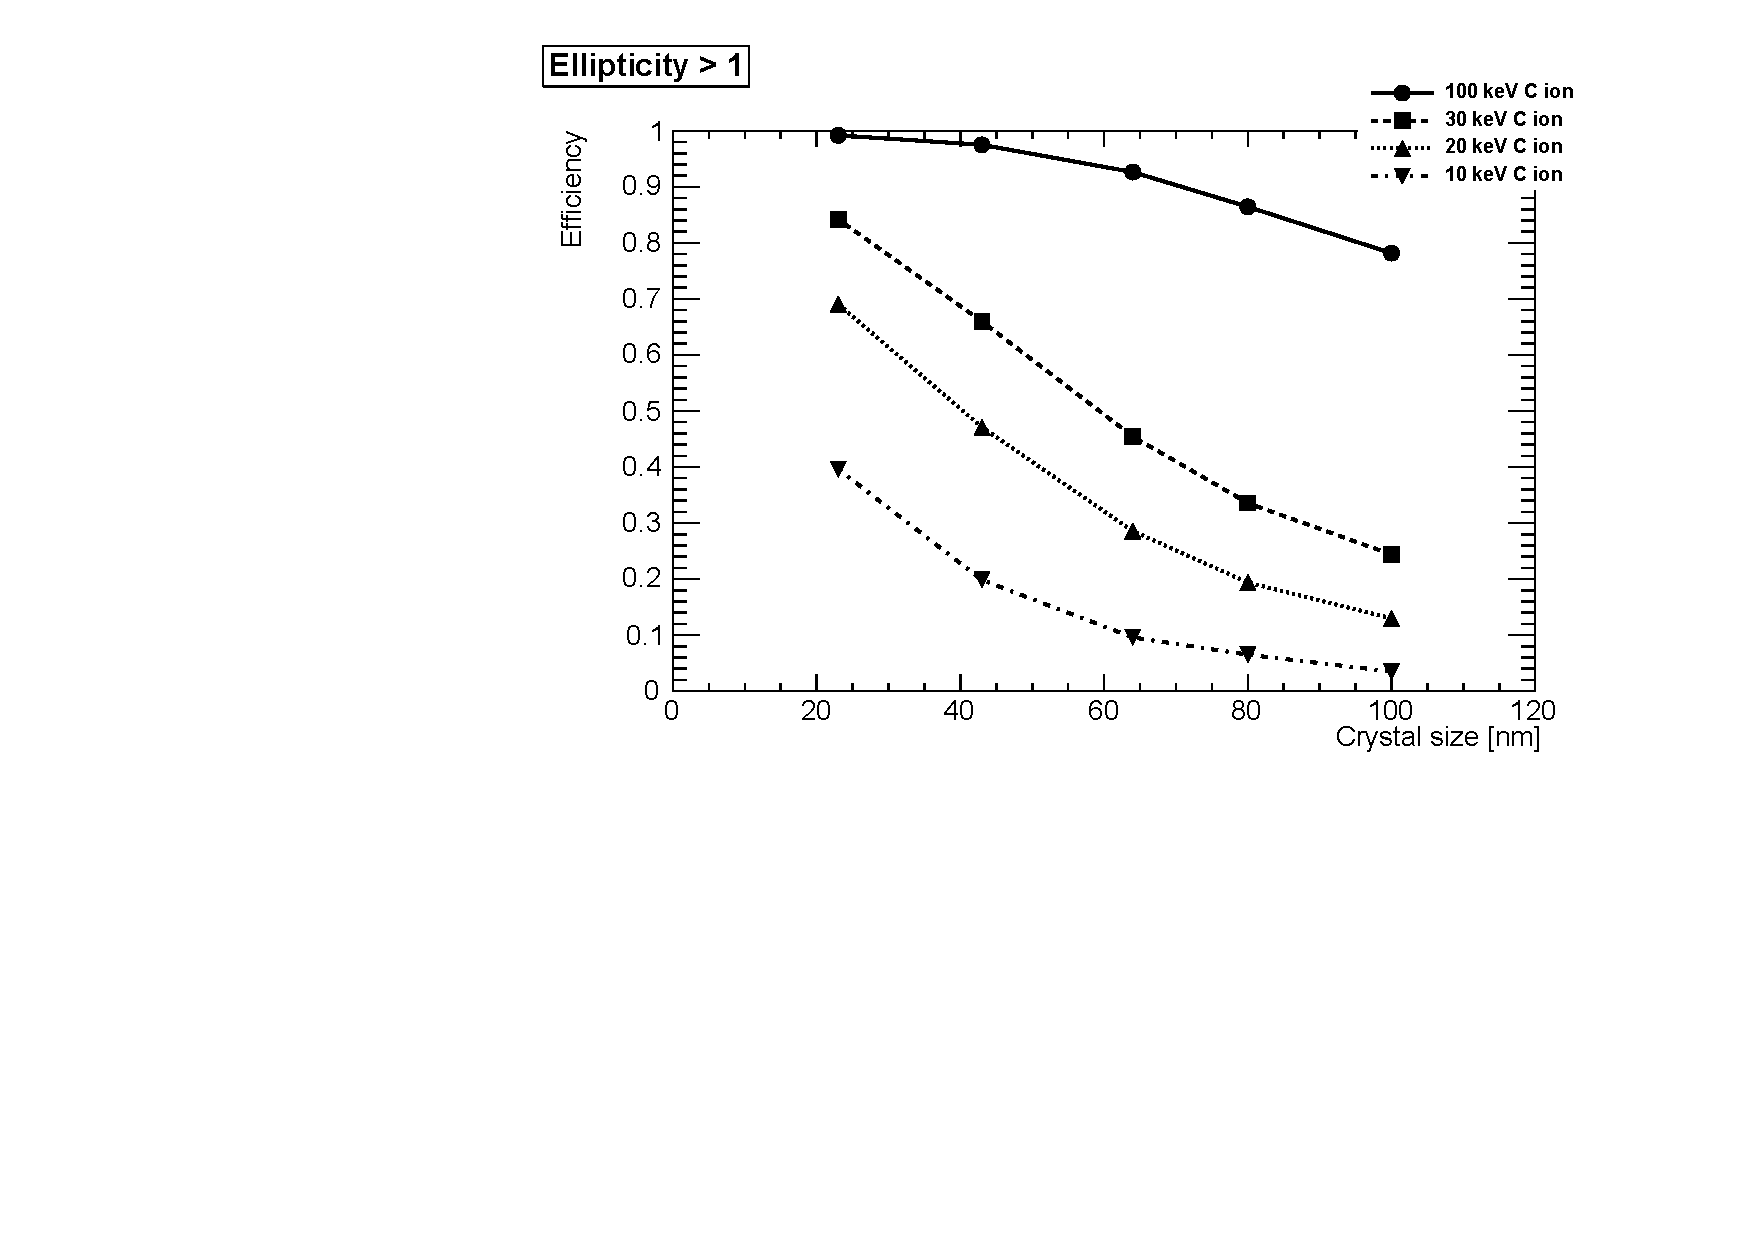
\includegraphics[angle=45,scale=0.2]{./figs/result2.pdf}}
\hspace{1em}
\subfloat[90~degree]{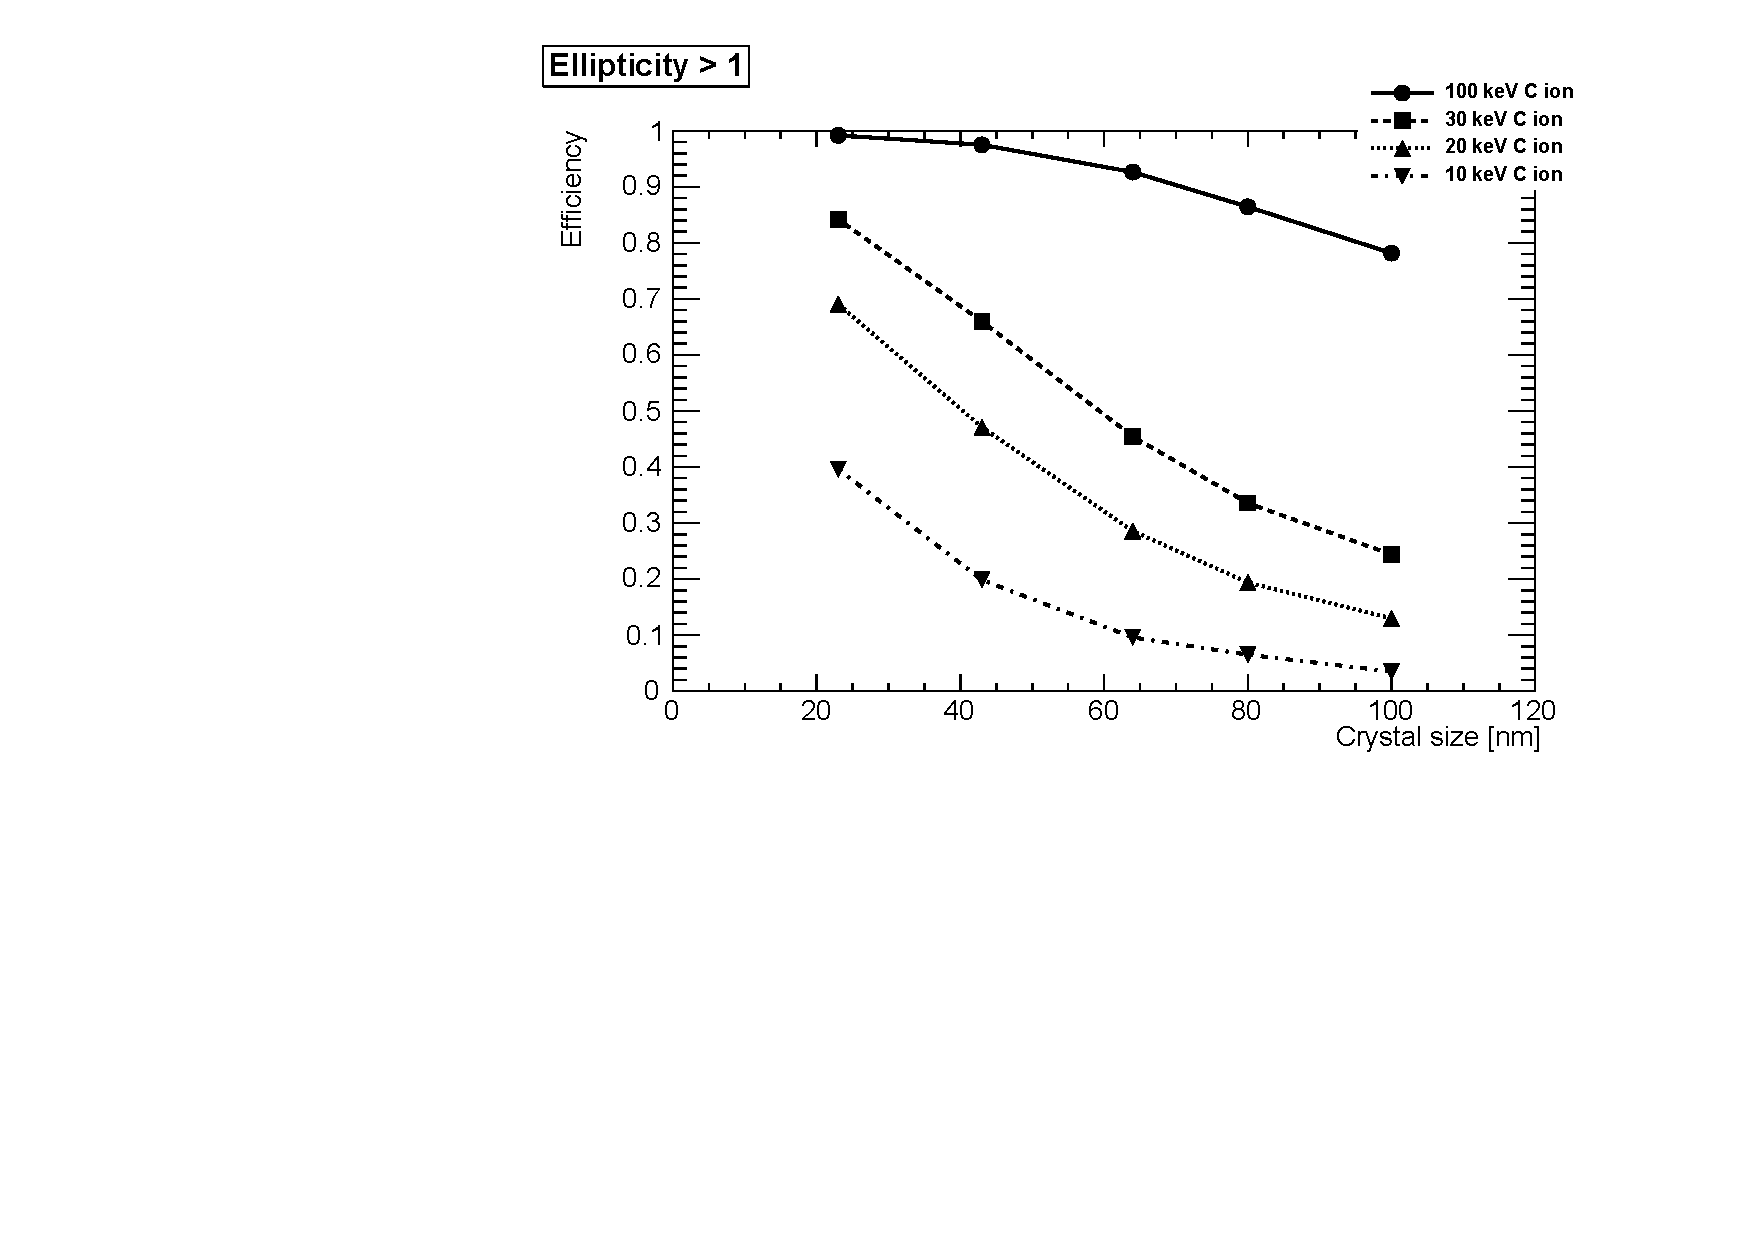
\includegraphics[angle=90,scale=0.2]{./figs/result2.pdf}}
\caption{画像を回転させたり、複数の画像を並べたりする方法\label{fig:multi_images}}
\end{figure}
\end{verbatim}

\begin{figure}[htbp]
\centering
\subfloat[0~degree]{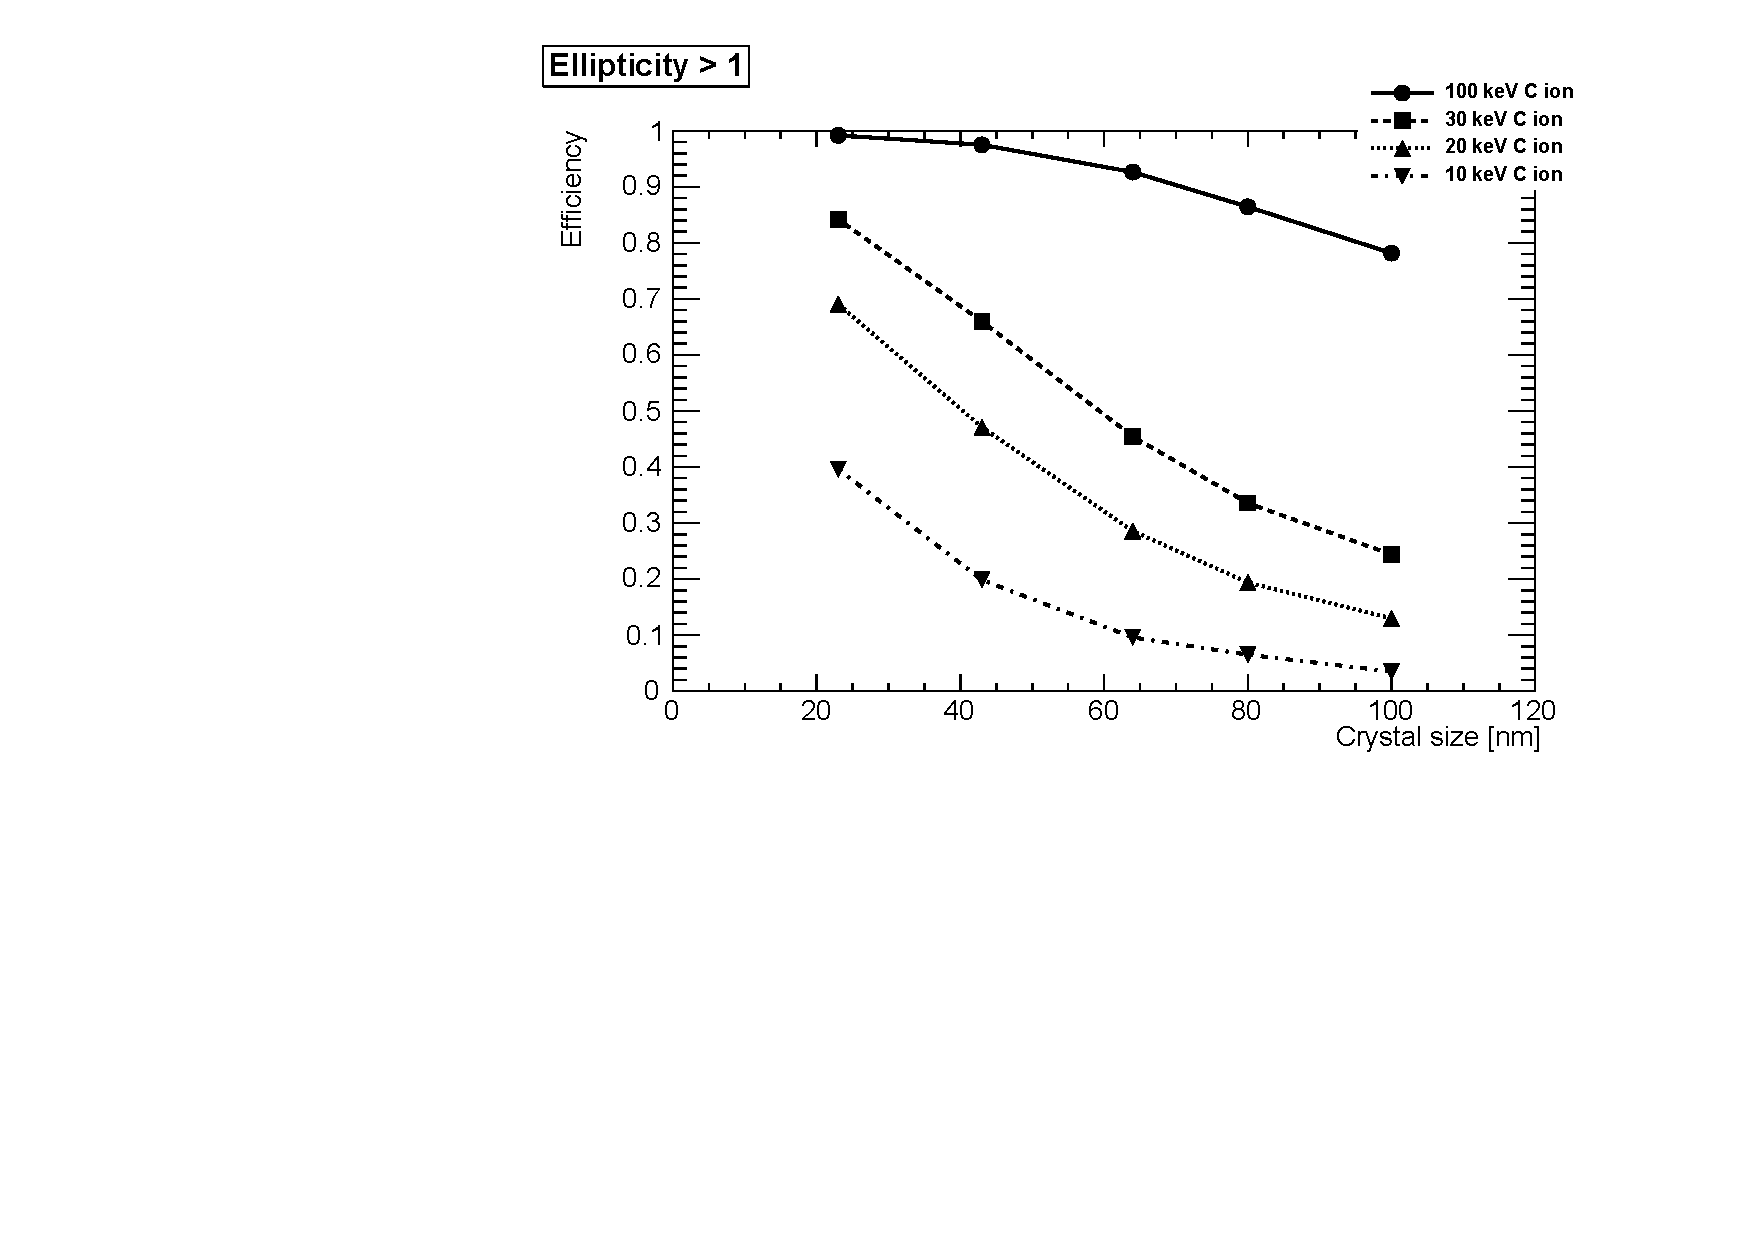
\includegraphics[angle=0,scale=0.2]{./figs/result2.pdf}}
\hspace{1em}
\subfloat[45~degree]{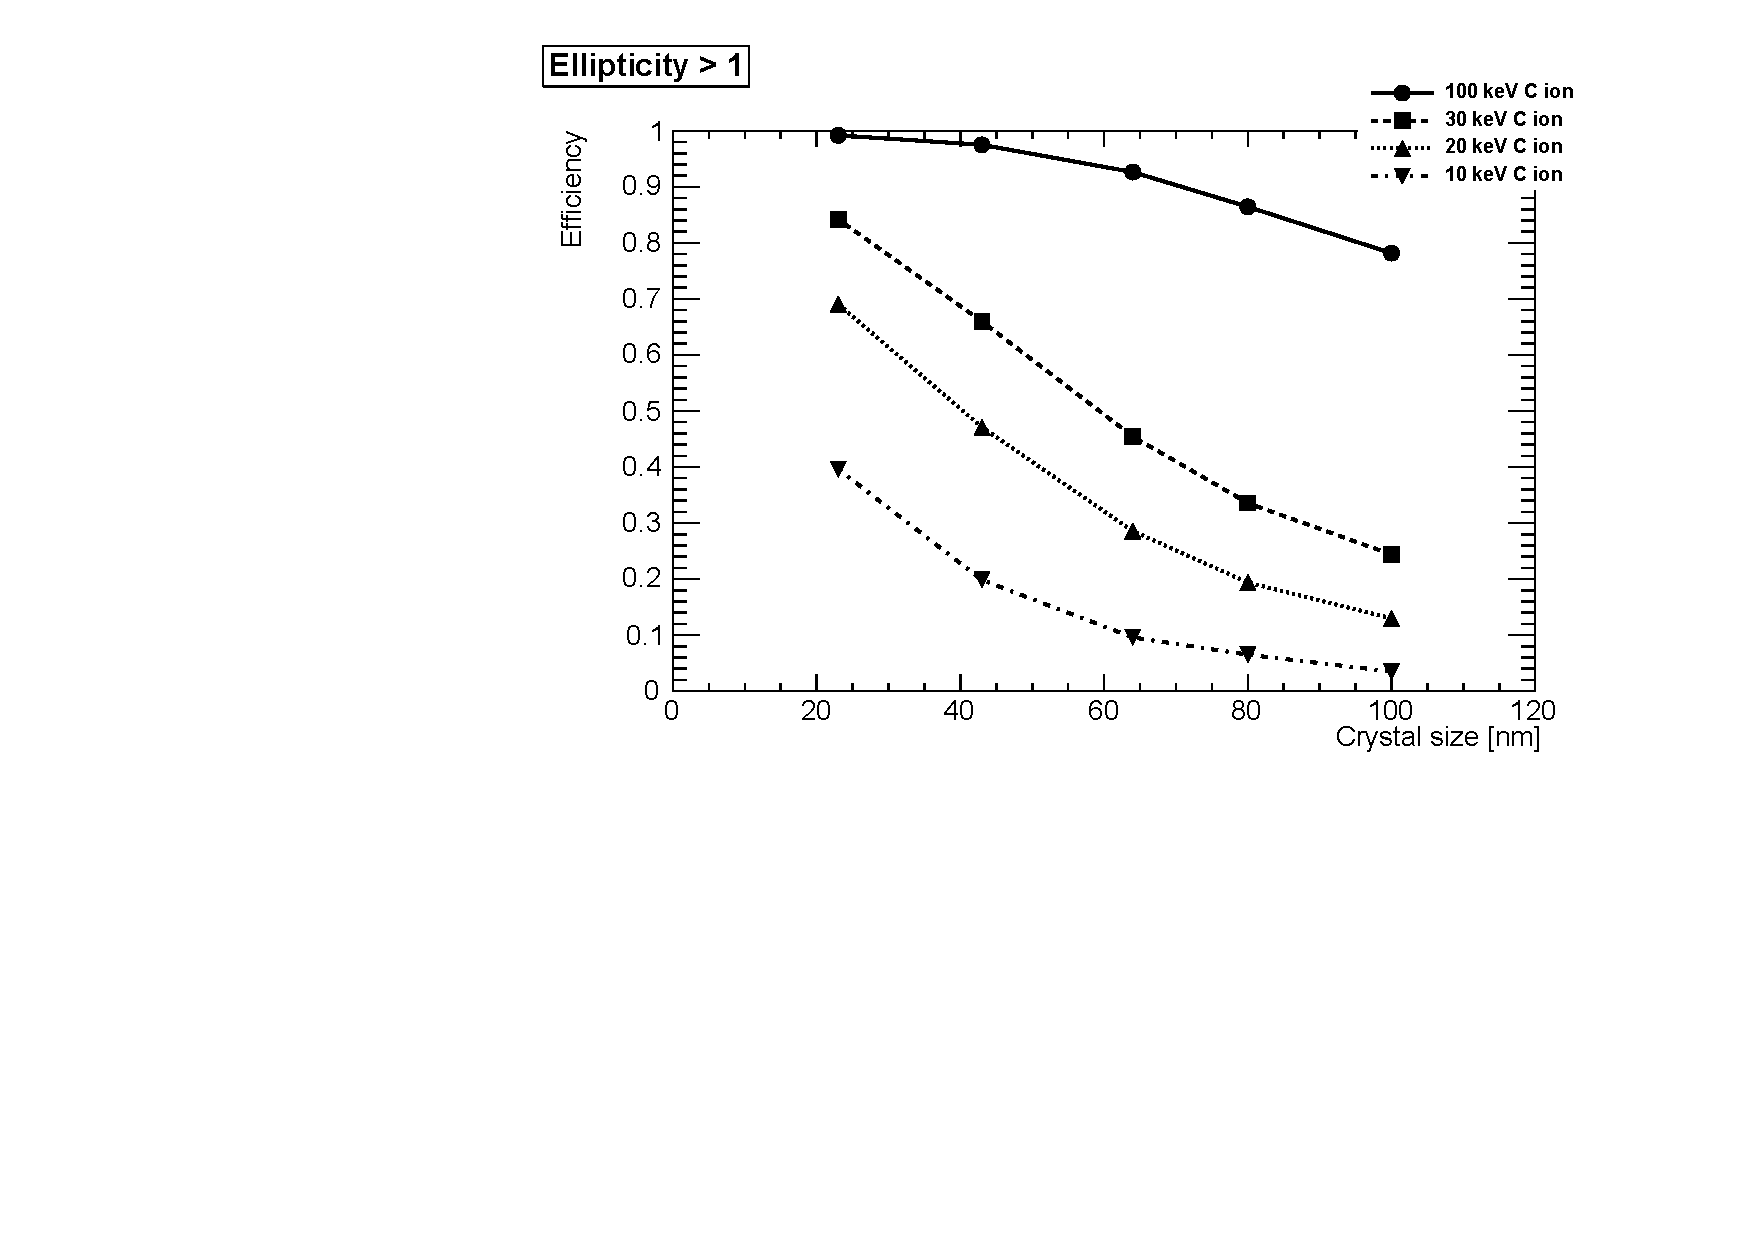
\includegraphics[angle=45,scale=0.2]{./figs/result2.pdf}}
\hspace{1em}
\subfloat[90~degree]{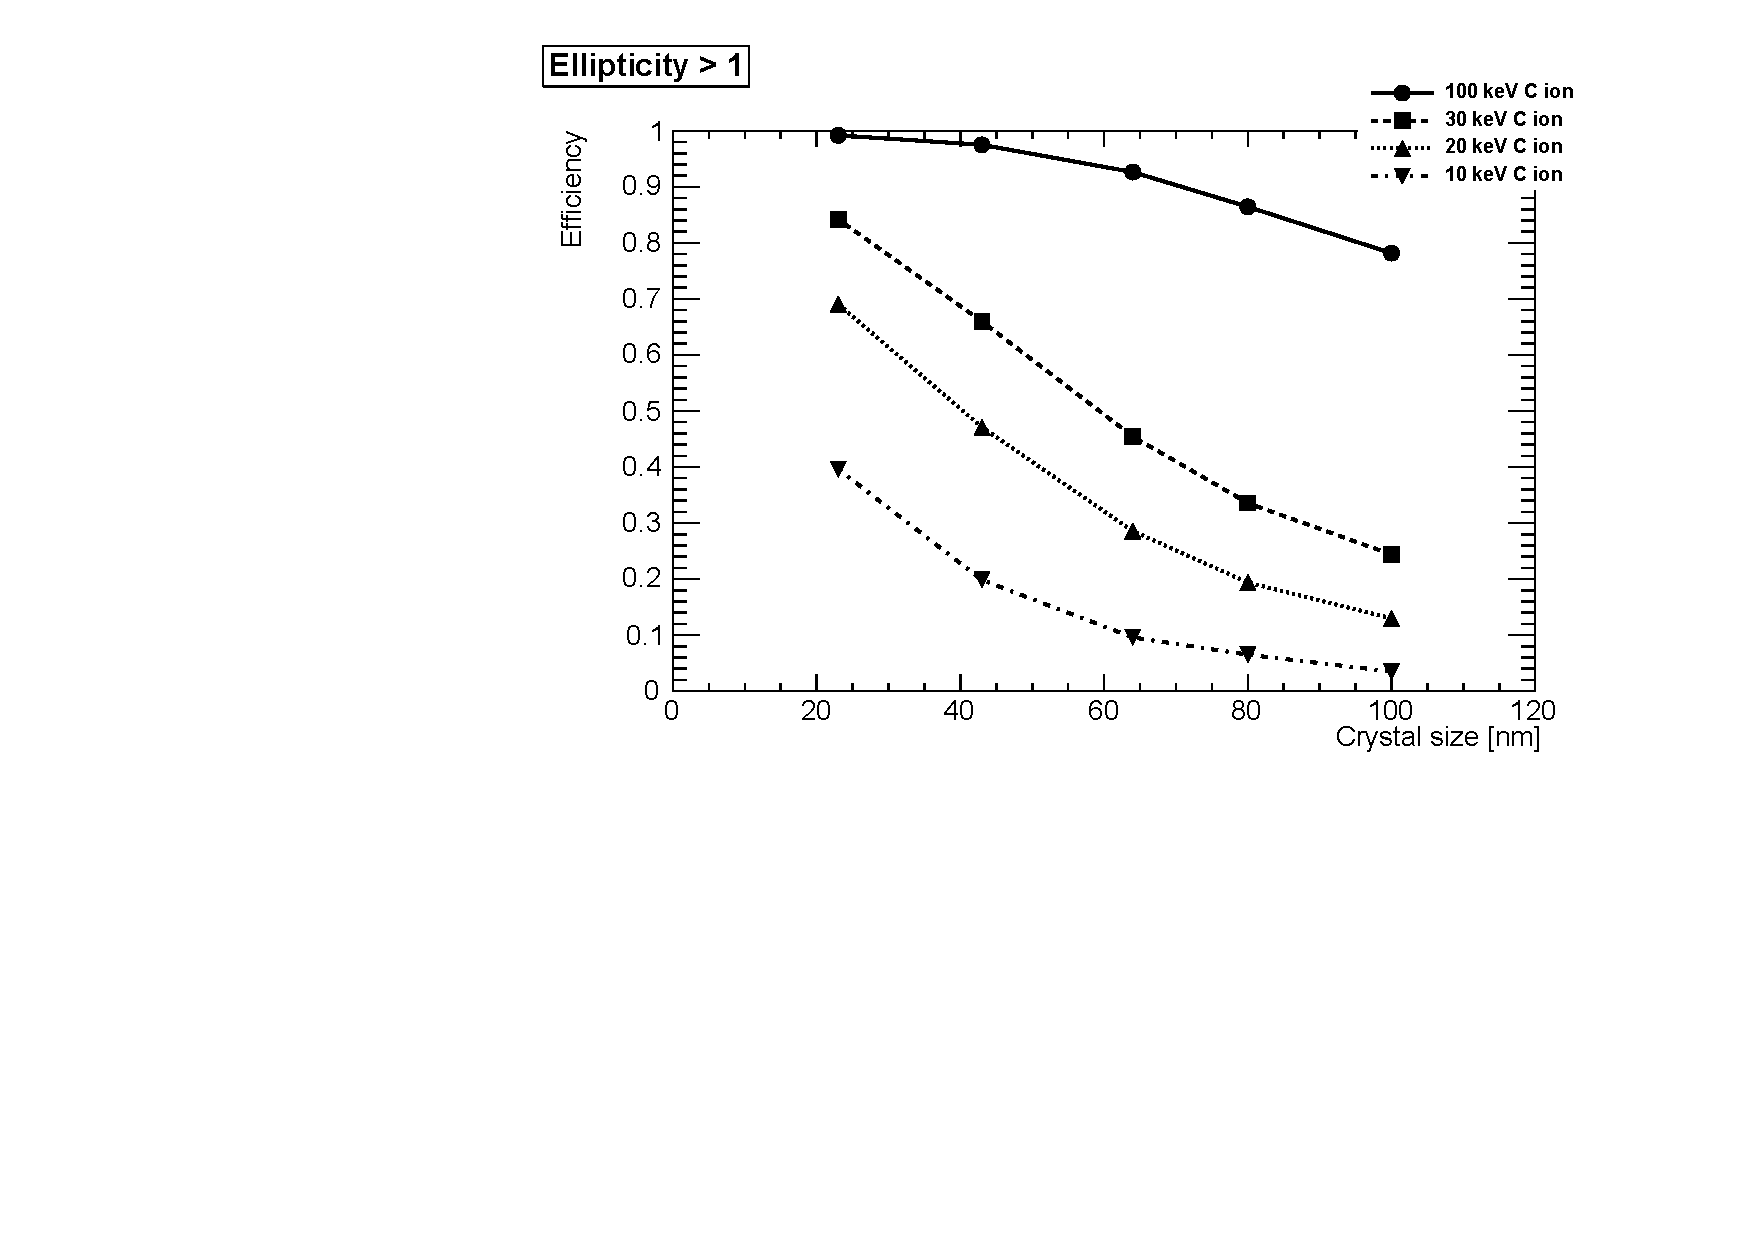
\includegraphics[angle=90,scale=0.2]{./figs/result2.pdf}}
\caption{画像を回転させたり、複数の画像を並べたりする方法\label{fig:multi_images}}
\end{figure}
    

\subsection{図の表示の応用}

グラフを作るときは、論文内で検索しやすいようにPDFファイルで保存しておくと良い。他の形式ももちろん使える。図~\ref{fig:various_img}で例を描画した。それぞれ異なる拡張子で表示してみた。
ちなみに、png、eps、jpgを使うときは\verb|\usepackage[dvipdfmx]{color}|が必要となる。検索すると分かるが、EPSファイルでは図内の文字が検索可能になっている。

\begin{figure}[htbp]
\centering
\subfloat[pngファイル]{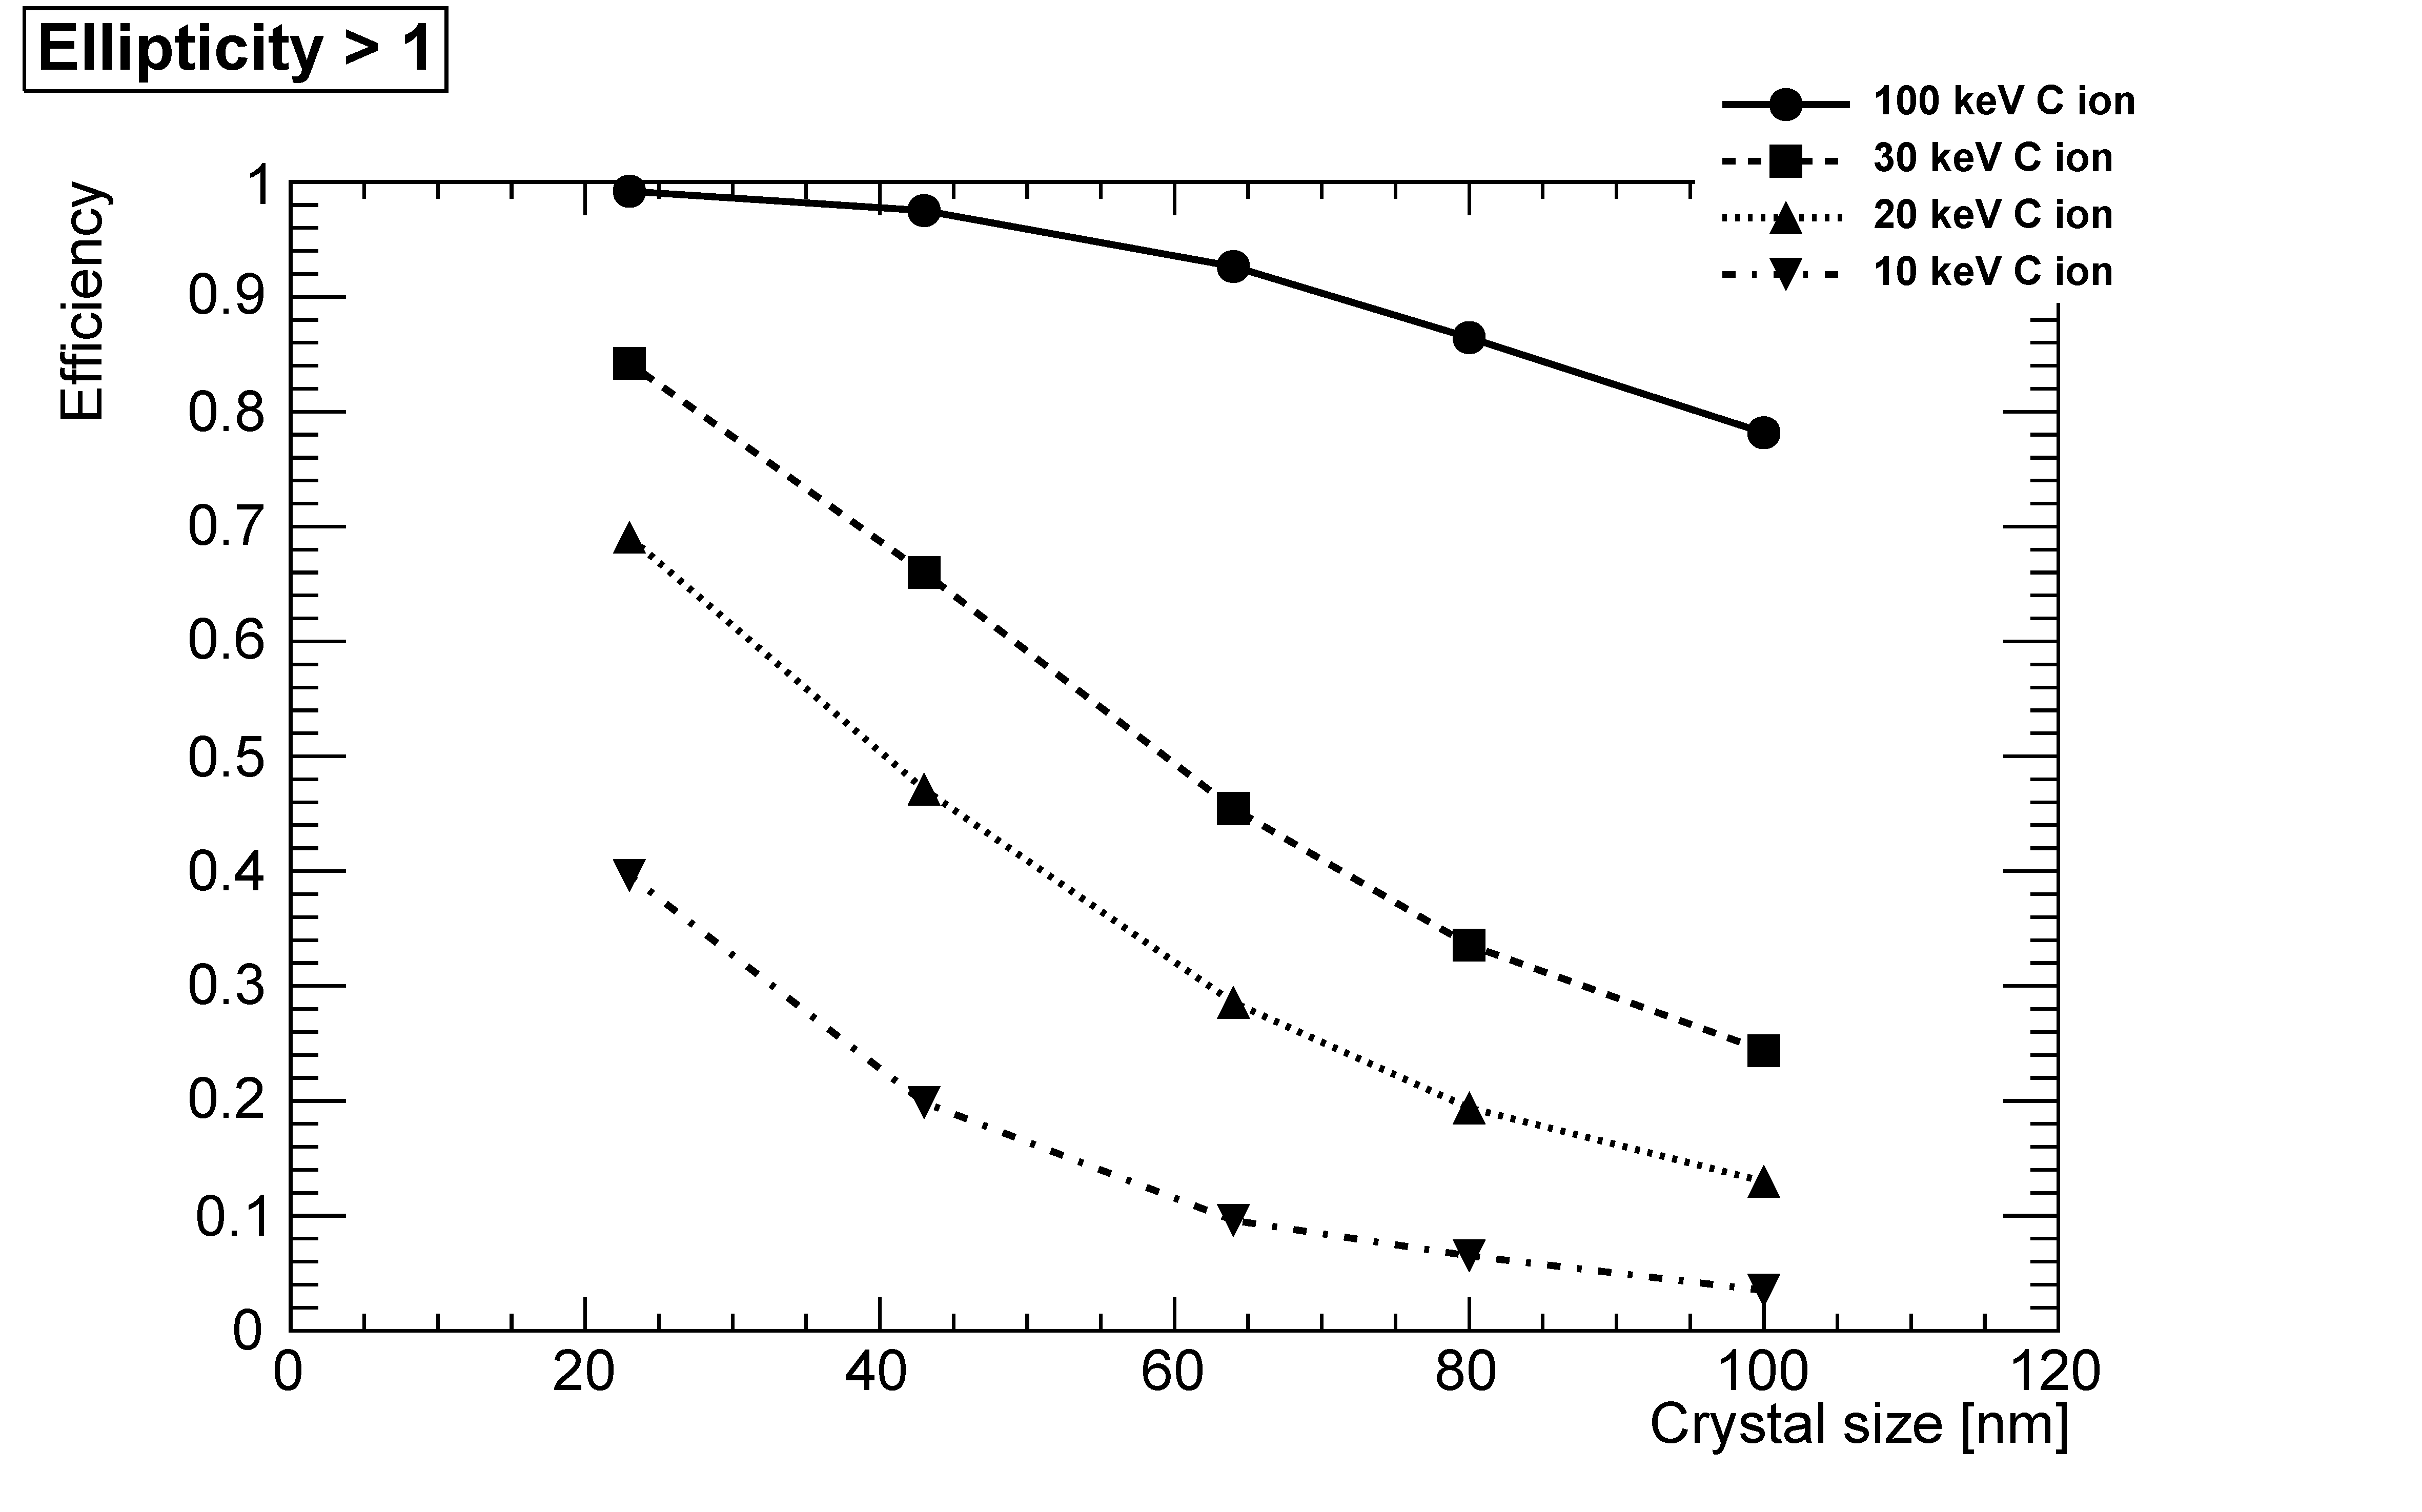
\includegraphics[scale=0.2]{./figs/result.png}}
\subfloat[epsファイル]{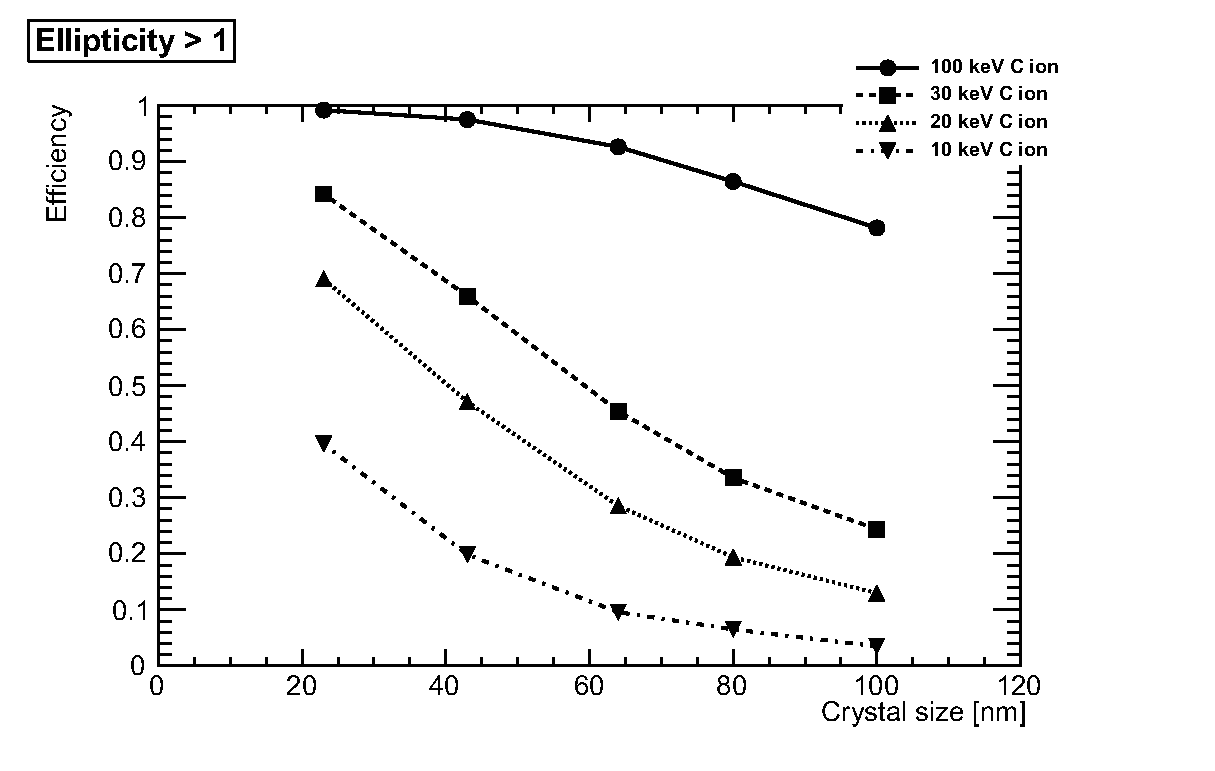
\includegraphics[scale=0.2]{./figs/result.eps}}
\subfloat[jpgファイル]{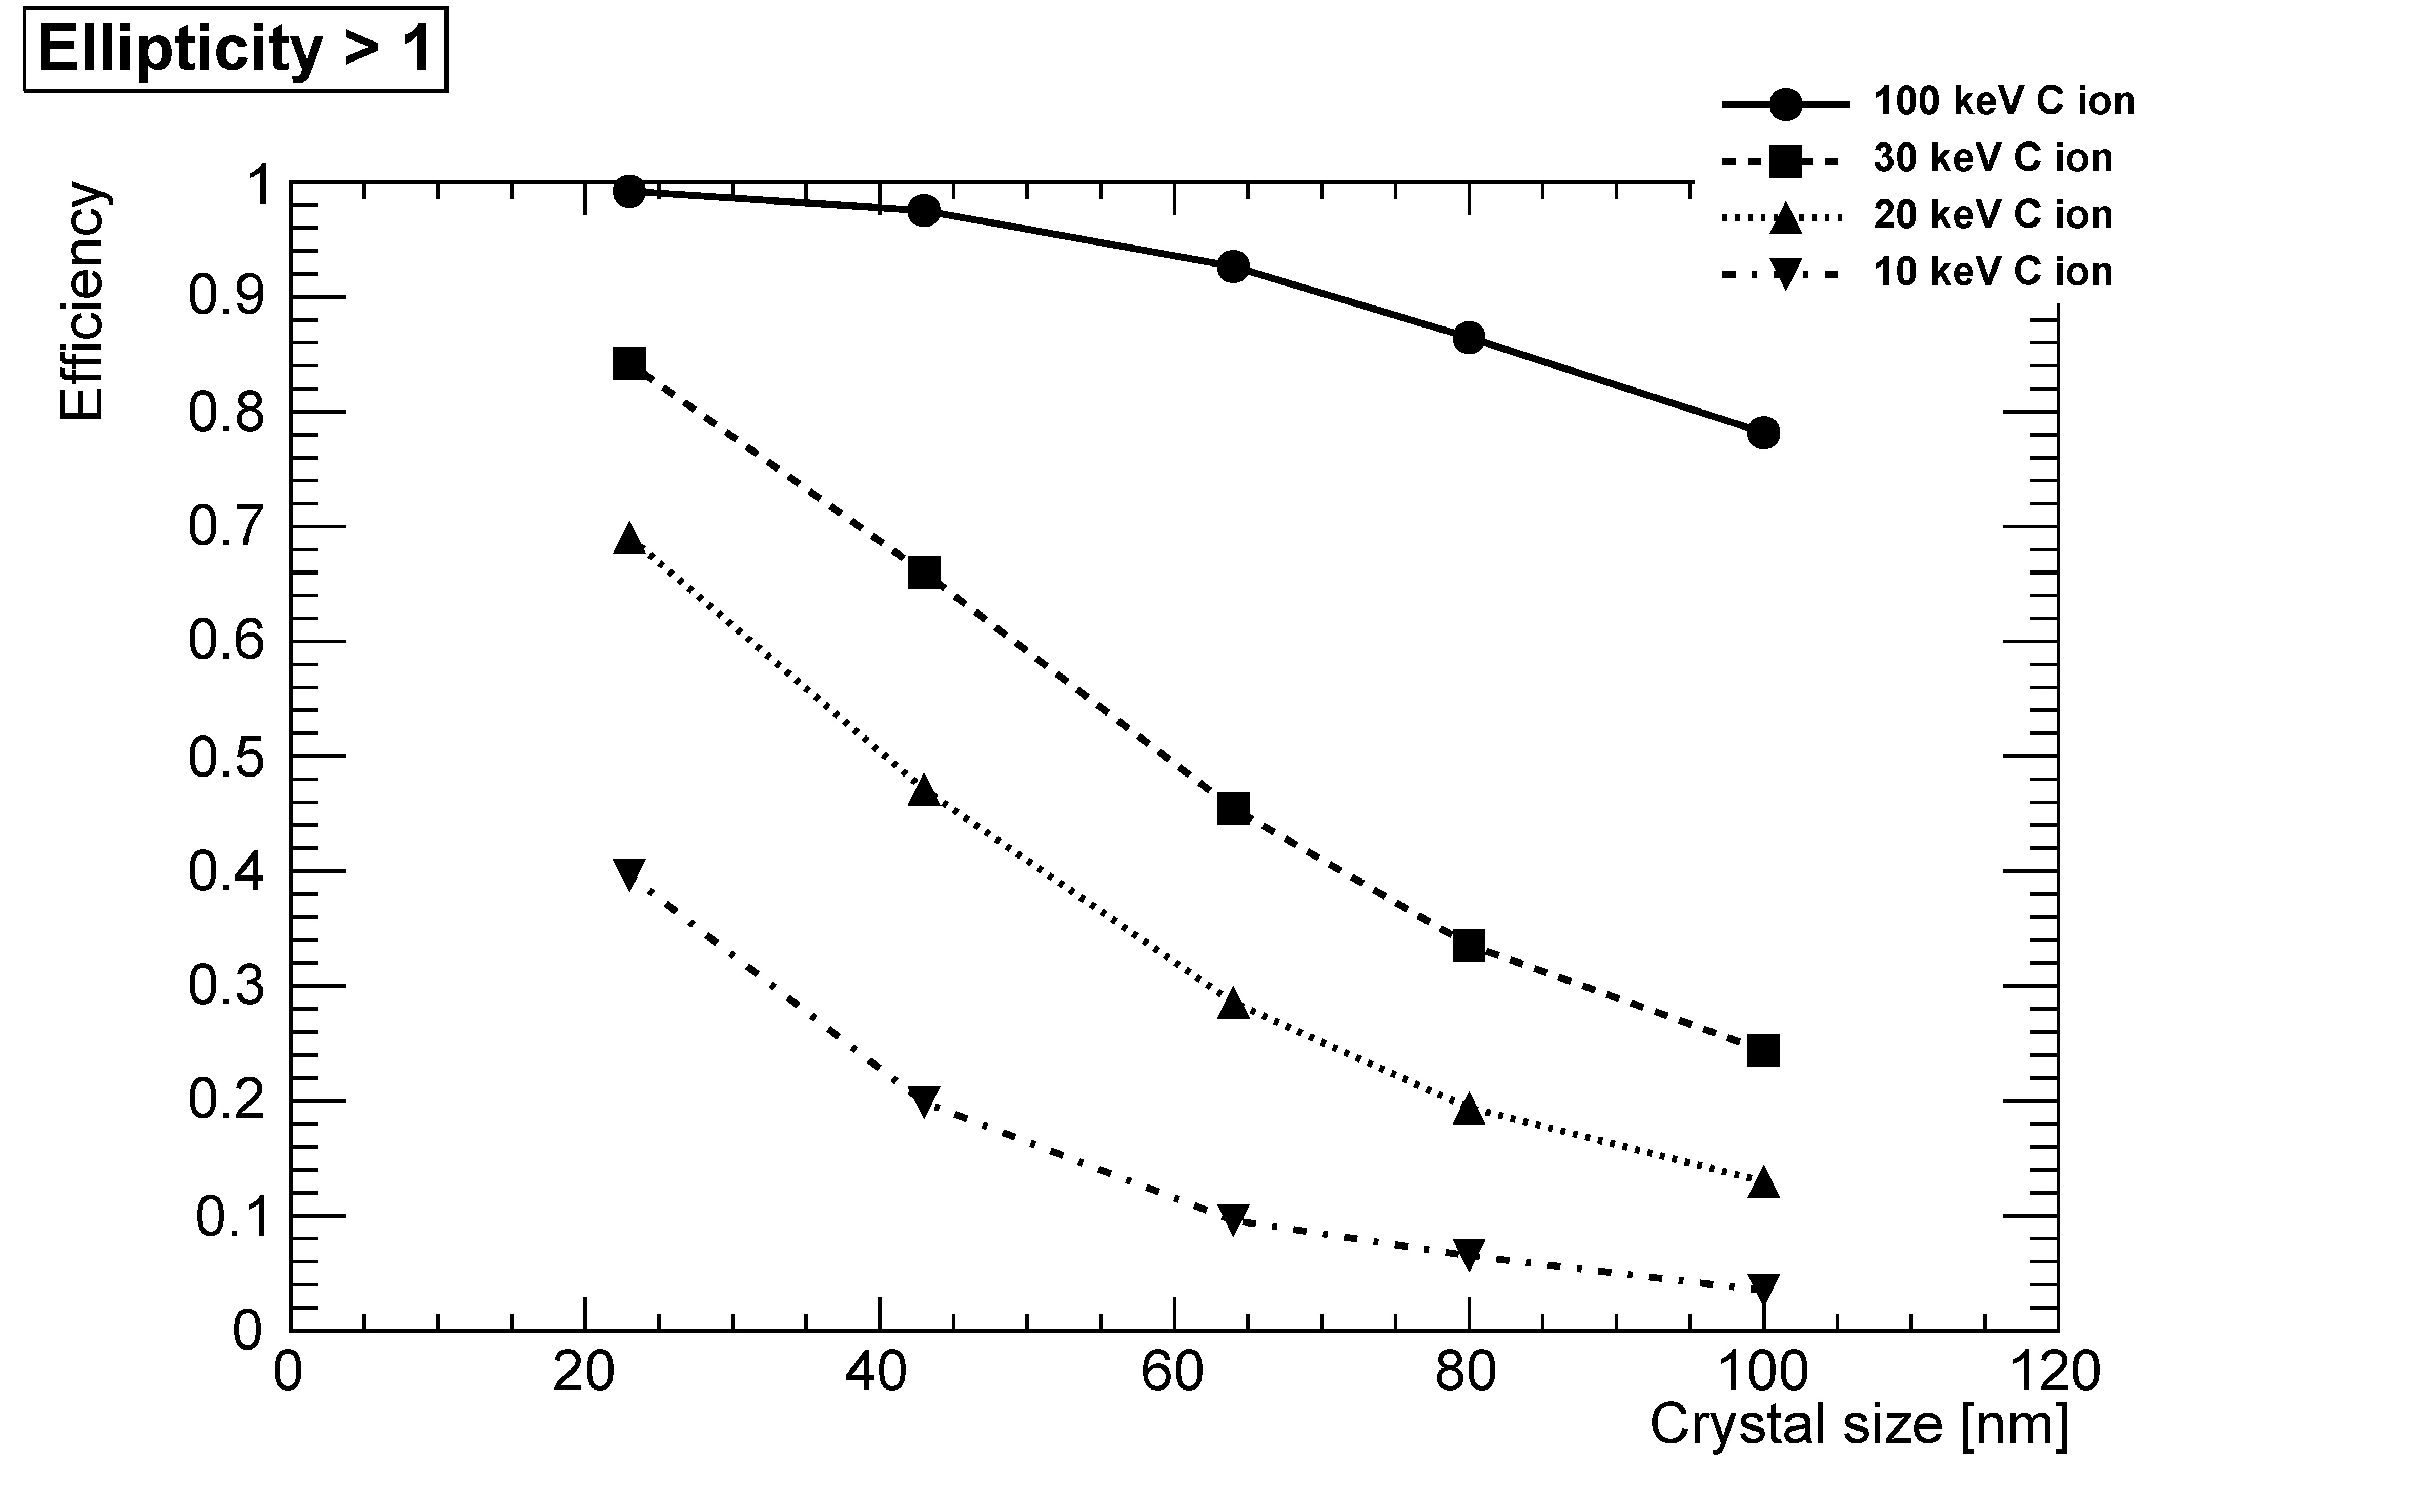
\includegraphics[scale=0.2]{./figs/result.jpg}}
\caption{png, eps, jpgの画像を表示する方法\label{fig:various_img}}
\end{figure}

機会は少ないとは思うが、複数ページを持つPDFはページ番号を指定して表示させることが可能である。図~\ref{fig:multi_page}で例を描画した。図~\ref{fig:page1}は1ページ目、図~\ref{fig:page2}は2ページ目。

\begin{figure}[htbp]
\centering
\subfloat[multi\_page.pdfの1ページ目 width=0.5\label{fig:page1}]
{\fbox{
\includegraphics[page=1,width=0.5\textwidth]{./figs/multi_page.pdf}}}
\hspace{1em}
\subfloat[multi\_page.pdfの2ページ目 width=0.3\label{fig:page2}]
{\fbox{
\includegraphics[page=2,width=0.3\textwidth]{./figs/multi_page.pdf}}}
\caption{複数ページを持つPDFの一部を表示させる方法\label{fig:multi_page}}
\end{figure}

\clearpage

\section{表(テーブル)}
\subsection{texにおける表の書き方}
表は、次の記述で表~\ref{tab:emulsion_telescope}のようになる。詳細はググってほしい。
\begin{verbatim}
\begin{table}[htbp]
\centering
\caption{表の例: GRAINEエマルション望遠鏡の基本性能とFermi-LATとの比較\label{tab:emulsion_telescope}}
\begin{tabular}{r||c|l}
右寄せ&中央寄せ&左寄せ\\
     &Fermi-LAT&GRAINE\\
\hline
\hline
角度分解能@100~MeV& 105~mrad (6.0$^\circ$ )   & 17~mrad (1.0$^\circ$ ) \\
@1~GeV           & 16~mrad(0.90$^\circ$ )    & 1.7~mrad(0.10$^\circ$) \\
検出エネルギー範囲 &20--300~MeV                 & 10~MeV--100~GeV        \\
偏光感度          &無                          &有                      \\
不感時間          &26.5~$\mu$sec (readout time)& 0\%                    \\
\hline
\end{tabular}
\end{table}
\end{verbatim}
\begin{table}[htbp]
\centering
\caption{表の例: GRAINEエマルション望遠鏡の基本性能とFermi-LATとの比較\label{tab:emulsion_telescope}}
\begin{tabular}{r||c|l}
右寄せ&中央寄せ&左寄せ\\
     &Fermi-LAT&GRAINE\\
\hline
\hline
角度分解能@100~MeV& 105~mrad (6.0$^\circ$ )   & 17~mrad (1.0$^\circ$ ) \\
@1~GeV           & 16~mrad(0.90$^\circ$ )    & 1.7~mrad(0.10$^\circ$) \\
検出エネルギー範囲 &20--300~MeV                 & 10~MeV--100~GeV        \\
偏光感度          &無                          &有                      \\
不感時間          &26.5~$\mu$sec (readout time)& 0\%                    \\
\hline
\end{tabular}
\end{table}

\subsection{Excelでテーブルを作ってtexに挿入する方法}
複雑なレイアウトの表を作るときは、texファイル上で格闘するよりもMicrosoft Excelなどで作成した方が楽なことが多い。
例えば、セル内で改行したいとき、右寄せ中央寄せなどを同じ列で異なる設定にしたいとき、罫線を好きな場所に引きたい時、セルを結合したいときなどである。

Excelで表を作成し、PDFファイルとして保存し、必要な場所だけを切り抜いて画像またはPDFファイルとして保存する。そのPDFファイル(画像)を\ref{sec:figure}で説明したように図として挿入する。そのとき、\verb|\begin{figure} ~~ \end{figure}| ではなく\verb|\begin{table} ~~ \end{table}| とすると、図~1、図~2ではなく、表~1、表~2と自動的に番号付けされる。

Excelからtexファイルに表を挿入はいくつかの工程が必要となる。
表~\ref{tab:table_cop}に各方法をまとめた。
pdfcropを使うときは、Perlというプログラムを事前にインストールする必要がある(WindowsユーザーだとStrawberry Perl)。

\begin{verbatim}
\begin{table}[htbp]
    \centering
    \caption{\LaTeX で表を作成する方法(これはLaTeX+PDF)\label{tab:table_cop}}
    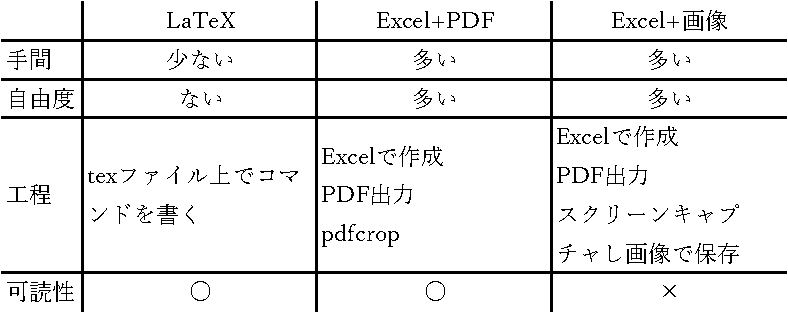
\includegraphics[width=110mm]{./figs/table_crop.pdf}
\end{table}
\end{verbatim}
\begin{table}[htbp]
    \centering
    \caption{\LaTeX で表を作成する方法(これはLaTeX+PDF)\label{tab:table_cop}}
    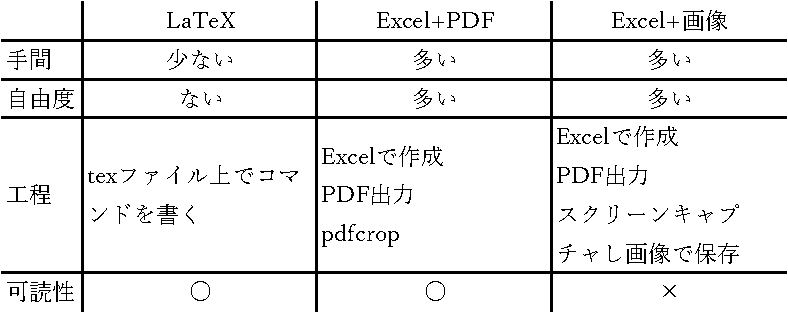
\includegraphics[width=110mm]{./figs/table_crop.pdf}
\end{table}
    
\clearpage
\section{リスト}
幾つかのリストを書く方法を示す。itemize, enumerate, descriptionがよく使われる。
\subsection{itemizeを使う方法}
\begin{verbatim}
\begin{itemize}
 \item 調液
 \item 粒子形成
 \item 水洗+脱塩
\end{itemize}
\end{verbatim}

\begin{itemize}
 \item 調液
 \item 粒子形成
 \item 水洗+脱塩
\end{itemize}
\subsection{descriptionを使う方法}
\begin{verbatim}
\begin{description}
 \item [調液]\mbox{} \\調液とは、
 \item [粒子形成]\mbox{} \\粒子形成とは、
 \item [水洗+脱塩]\mbox{} \\水洗と脱塩とは、
\end{description}
\end{verbatim}
\begin{description}
 \item [調液]\mbox{} \\調液とは、
 \item [粒子形成]\mbox{} \\粒子形成とは、
 \item [水洗+脱塩]\mbox{} \\水洗と脱塩とは、
\end{description}
\subsection{enumerateを使う方法}
原子核乳剤の主な原料は・・・番号を1番以外から始めたいときは\verb|\setcounter{enumi}{X}|を使う。
\begin{verbatim}
\begin{enumerate}
\setcounter{enumi}{10}
 \item 硝酸銀 (高い)
 \item 臭化カリウム
\end{enumerate}
\end{verbatim}
\begin{enumerate}
\setcounter{enumi}{10}
 \item 硝酸銀 (高い)
 \item 臭化カリウム
\end{enumerate}
\newpage
\section{数式}
equation*コマンドで数式を書くとただの数式を書ける。
\begin{verbatim}
\begin{equation*}
a=b
\end{equation*}
\end{verbatim}
\begin{equation*}
a=b
\end{equation*}
equationコマンドで数式を書くと番号が付く。式~\ref{equ:ab}で例を示す。
\begin{verbatim}
\begin{equation}
a=b
\label{equ:ab}
\end{equation}
\end{verbatim}
\begin{equation}
a=b
\label{equ:ab}
\end{equation}
一粒子系のシュレーディンガー方程式を式~\ref{equ:oneparticle}で示す。
\begin{verbatim}
\begin{equation}
i\hbar\frac{\partial}{\partial t} \psi(\boldsymbol{x},t) = 
\left [ \frac{-\hbar^2}{2m}\nabla^2 + V(\boldsymbol{x},t)\right ] \psi(\boldsymbol{x},t)
\label{equ:oneparticle}
\end{equation}
\end{verbatim}
\begin{equation}
i\hbar\frac{\partial}{\partial t} \psi(\boldsymbol{x},t) = 
\left [ \frac{-\hbar^2}{2m}\nabla^2 + V(\boldsymbol{x},t)\right ] \psi(\boldsymbol{x},t)
\label{equ:oneparticle}
\end{equation}

\subsection{上付き下付き文字}
\begin{verbatim}
$x^a, x^{a+b}, x^{a^b}, a_i, a_{ij}, a_{i_j}$
\end{verbatim}
$x^a, x^{a+b}, x^{a^b}, a_i, a_{ij}, a_{i_j}$

\subsection{不等号}
\begin{verbatim}
$\sim, \simeq, >, <, \geq, \leq, \gg, \ll$
\end{verbatim}
$\sim, \simeq, >, <, \geq, \leq, \gg, \ll$

\subsection{演算子}
\begin{verbatim}
$+, -, \times, \div, \pm, \mp, \circ, \cdot$
\end{verbatim}
$+, -, \times, \div, \pm, \mp, \circ, \cdot$

\subsection{平方根}
\begin{verbatim}
$\sqrt{x}, \sqrt[n]{x}$
\end{verbatim}
$\sqrt{x}, \sqrt[n]{x}$

\subsection{ギリシャ文字}
\begin{verbatim}
$\Gamma, \Delta, \Theta, \Lambda, \Xi, \Pi, \Sigma, \Upsilon, \Phi, \Psi, \Omega$
\end{verbatim}
$\Gamma, \Delta, \Theta, \Lambda, \Xi, \Pi, \Sigma, \Upsilon, \Phi, \Psi, \Omega$

\begin{verbatim}
$\alpha, \beta, \gamma, \delta, \epsilon, \zeta, \eta, \theta, \iota, \kappa, \lambda, $\\
$\mu, \nu, $\xi, o, \pi, \rho, \sigma, \tau, \upsilon, \phi, \chi, \psi, \omega, $
\end{verbatim}
$\alpha, \beta, \gamma, \delta, \epsilon, \zeta, \eta, \theta, \iota, \kappa, \lambda, $\\
$\mu, \nu, \xi, o, \pi, \rho, \sigma, \tau, \upsilon, \phi, \chi, \psi, \omega, $
\subsection{行列}
\begin{verbatim}
\begin{equation}
 \begin{array}{rrr}
-1 & \ldots & 3 \\
\vdots & \ddots & 600 \\
  7 & 8 & -9
 \end{array}
\end{equation}
\end{verbatim}

\begin{equation}
\begin{array}{rrr}
-1 & \ldots & 3 \\
\vdots & \ddots & 600 \\
7 & 8 & -9
\end{array}
\end{equation}
\subsection{括弧}
\verb|\left \right|を使うと\verb|[ ], ( ), { }, | $|\;|$等で囲まれる数式を正しく囲むことができる。
\begin{verbatim}
\begin{equation}
 \left [ \frac{0}{1} \right ] + [\frac{0}{1}]
\end{equation}
\end{verbatim}
\begin{equation}\left [ \frac{0}{1} \right ] + [\frac{0}{1}]\end{equation}
\subsection{数式中の空白や改行}
数式モードでは全ての空白は無視されるので、明示的に空白コマンドを使う。改行して=でそろえたい場合は\verb|\begin{split}\end{split}|を使い、\verb|\\|で改行、\verb|&|でそろえる場所を指定する。
\begin{verbatim}
\begin{equation}
\begin{split}
a&=|\;| 大きめの空白\\
b&=|\:| 中くらいの空白\\
c&=|\,| 小さめの空白\\
d&=|| 空白なし\\
e&=|\!| 負の空白
\end{split}
\end{equation}
\end{verbatim}
\begin{equation}
\begin{split}
a&=|\;| 大きめの空白\\
b&=|\:| 中くらいの空白\\
c&=|\,| 小さめの空白\\
d&=|| 空白なし\\
e&=|\!| 負の空白
\end{split}
\end{equation}
\subsection{総和・総乗}
\begin{verbatim}
\begin{equation} f(x) = \sum_{i=0}^n x_i \end{equation}

\begin{equation}  f(x) = \prod_{i=0}^n x_i \end{equation}
\end{verbatim}
\begin{equation} f(x) = \sum_{i=0}^n x_i \end{equation}

\begin{equation}  f(x) = \prod_{i=0}^n x_i \end{equation}
\subsection{頻出表現}
\label{sec:frequent}
\noindent
角度 $^\circ$ = \verb|$^\circ$|\\
ミクロン $\mu m$ = \verb|$\mu m$|\\
数式中で斜体にしない $\rm{mm}$ = \verb|$\rm{mm}$|\\
ニュートリノ振動 $\nu_{\mu} \rightarrow \nu_{\tau}$ = \verb|$\nu_{\mu} \rightarrow \nu_{\tau}$|\\
臭化銀の沈殿 $\rm{KBr+AgNO_3\rightarrow AgBr\downarrow+KNO_3}$ = \verb|$\rm{KBr+AgNO_3\rightarrow AgBr\downarrow+KNO_3}$|\\
ハイパー核$_{\Lambda\Lambda}^{~6}$He = \verb|$_{\Lambda\Lambda}^{~6}$He|\\
レイリーの基準$\delta x = 0.61\frac{\lambda}{\rm{NA}}$ = \verb|$\delta x = 0.61\frac{\lambda}{\rm{NA}}$|\\
ベクトル $\overrightarrow{ma}$ = \verb|$\overrightarrow{ma}$|\\
三角関数 $\sin\theta \cos\phi \tan\alpha$ = \verb|$\sin\theta \cos\phi \tan\alpha$|

\subsection{Tips}
Wikipediaの数式は\LaTeX の数式表記になっているので、欲しい関数は編集からソースを見るとよい。一粒子系のシュレーディンガー方程式もWikipediaからのコピペである。
\newpage
\section{その他}
\subsection{URL}
\verb|\begin{document}|の前に\verb|\usepackage{url}|が必要。
\begin{verbatim}
\url{https://www1.gifu-u.ac.jp/~physics/}
\end{verbatim}
\url{https://www1.gifu-u.ac.jp/~physics/}

\subsection{参照}
論文の参照は\verb|\cite{}|を用いる、\ref{sec:figure}で説明したが、図、表、数式、セクションの参照は\verb|\ref{}|を用いる。図、表、数式などはそれぞれ1から順番に出現した順番に番号が振られる。他の図などをコピペしたときにlabelの書き換え忘れが頻繁に発生するので注意してほしい。
\begin{verbatim}
私の博士論文の副論文~\cite{Yoshimoto:2017ufm}、論文を探すにはinspire~\cite{inspire}やGoogle Scholar~\cite{google-scholar}、頻出表現は\ref{sec:frequent}を参照せよ。
\end{verbatim}
私の博士論文の副論文~\cite{Yoshimoto:2017ufm}、論文を探すにはinspire~\cite{inspire}やGoogle Scholar~\cite{google-scholar}、頻出表現は\ref{sec:frequent}を参照せよ。

\subsection{他のページを読み込む}
別のファイルに中身を書いておいて、それをメインのファイルに統合することができる。inputはそのまま代入され、includeは読み込んだファイルの直前で改ページされる。拡張子\verb|.tex|は必要ない。
\begin{verbatim}
\input{abst}
\include{abst}
\end{verbatim}

\subsection{丸付き文字}
通常の論文で丸付き文字を使うことはないが、使う場合は
\textcircled{\scriptsize 1} = \verb|\textcircled{\scriptsize 1}|\\ とする。
科研費などで次のようにも書ける。\verb|\raise0.2ex\hbox{\textcircled{\scriptsize{3}}}|

\subsection{文章を強調する}
通常の論文で文章を強調することはないが、使いたい場合は次のようにする。

\noindent
\underline{下線を引いたり} = \verb|\underline{下線を引いたり}|\\
{\bf 太字にしたり} = \verb|{\bf 太字にしたり}|\\
\colorbox[named]{Black}{\color[named]{White}{\bf 黒背景にしたり}} = \verb|\colorbox[named]{Black}{\color[named]{White}{\bf 黒背景にしたり}}|\\
科研費や学振の場合、白黒印刷されるらしいので、基本的に白黒で強調すると良いだろう。 下線はその途中で改行できないので注意せよ。

\subsection{PDF内のリンクについて}
PDFファイルを見ると、所々で色付きの□が表示されている。そこをクリックすると、セクションや図、表、参考文献などに飛んでくれる。
この□は印刷するときには表示されないので心配無用である。

\subsection{表目次、図目次、参考文献}
表目次\verb|\listoftables|、図目次\verb|\listoffigures|と書けば、そこに各目次が表示される。最後に書くと良いだろう。
参考文献はややこしいのでソースをみてほしい。
%\newpage %新しいページ
\listoftables %テーブルリスト
%\newpage %新しいページ
\listoffigures %図のリスト

\begin{thebibliography}{99}
\bibitem{Yoshimoto:2017ufm} 
  M.~Yoshimoto, T.~Nakano, R.~Komatani and H.~Kawahara,
  ``Hyper-track selector nuclear emulsion readout system aimed at scanning an area of one thousand square meters,''
  PTEP {\bf 2017}, no. 10, 103H01 (2017)
  % doi:10.1093/ptep/ptx131
  % [arXiv:1704.06814 [physics.ins-det]].
  %%CITATION = doi:10.1093/ptep/ptx131;%%
  %9 citations counted in INSPIRE as of 31 Oct 2018
\bibitem{inspire}
\url{https://inspirehep.net/}
\bibitem{google-scholar}
\url{https://scholar.google.co.jp/}
\end{thebibliography}

\end{document}
